% Options for packages loaded elsewhere
\PassOptionsToPackage{unicode}{hyperref}
\PassOptionsToPackage{hyphens}{url}
%
\documentclass[
]{article}
\usepackage{lmodern}
\usepackage{amssymb,amsmath}
\usepackage{ifxetex,ifluatex}
\ifnum 0\ifxetex 1\fi\ifluatex 1\fi=0 % if pdftex
  \usepackage[T1]{fontenc}
  \usepackage[utf8]{inputenc}
  \usepackage{textcomp} % provide euro and other symbols
\else % if luatex or xetex
  \usepackage{unicode-math}
  \defaultfontfeatures{Scale=MatchLowercase}
  \defaultfontfeatures[\rmfamily]{Ligatures=TeX,Scale=1}
\fi
% Use upquote if available, for straight quotes in verbatim environments
\IfFileExists{upquote.sty}{\usepackage{upquote}}{}
\IfFileExists{microtype.sty}{% use microtype if available
  \usepackage[]{microtype}
  \UseMicrotypeSet[protrusion]{basicmath} % disable protrusion for tt fonts
}{}
\makeatletter
\@ifundefined{KOMAClassName}{% if non-KOMA class
  \IfFileExists{parskip.sty}{%
    \usepackage{parskip}
  }{% else
    \setlength{\parindent}{0pt}
    \setlength{\parskip}{6pt plus 2pt minus 1pt}}
}{% if KOMA class
  \KOMAoptions{parskip=half}}
\makeatother
\usepackage{xcolor}
\IfFileExists{xurl.sty}{\usepackage{xurl}}{} % add URL line breaks if available
\IfFileExists{bookmark.sty}{\usepackage{bookmark}}{\usepackage{hyperref}}
\hypersetup{
  pdftitle={Survival Analysis of Post-Myocardial Infarction Patients},
  pdfauthor={Research: Alvein, Parametric: Orr, Non-Parametric: Pham},
  hidelinks,
  pdfcreator={LaTeX via pandoc}}
\urlstyle{same} % disable monospaced font for URLs
\usepackage[margin=1in]{geometry}
\usepackage{graphicx,grffile}
\makeatletter
\def\maxwidth{\ifdim\Gin@nat@width>\linewidth\linewidth\else\Gin@nat@width\fi}
\def\maxheight{\ifdim\Gin@nat@height>\textheight\textheight\else\Gin@nat@height\fi}
\makeatother
% Scale images if necessary, so that they will not overflow the page
% margins by default, and it is still possible to overwrite the defaults
% using explicit options in \includegraphics[width, height, ...]{}
\setkeys{Gin}{width=\maxwidth,height=\maxheight,keepaspectratio}
% Set default figure placement to htbp
\makeatletter
\def\fps@figure{htbp}
\makeatother
\setlength{\emergencystretch}{3em} % prevent overfull lines
\providecommand{\tightlist}{%
  \setlength{\itemsep}{0pt}\setlength{\parskip}{0pt}}
\setcounter{secnumdepth}{-\maxdimen} % remove section numbering
\usepackage{booktabs}
\usepackage{longtable}
\usepackage{array}
\usepackage{multirow}
\usepackage{wrapfig}
\usepackage{float}
\usepackage{colortbl}
\usepackage{pdflscape}
\usepackage{tabu}
\usepackage{threeparttable}
\usepackage{threeparttablex}
\usepackage[normalem]{ulem}
\usepackage{makecell}
\usepackage{xcolor}

\title{Survival Analysis of Post-Myocardial Infarction Patients}
\author{Research: Alvein, Parametric: Orr, Non-Parametric: Pham}
\date{5/22/2020}

\begin{document}
\maketitle

\hypertarget{abstract}{%
\section{Abstract}\label{abstract}}

\(\textbf{Background:}\) The rates of myocardial infarction is becoming
an increasing common occurrence in the United States. Rapid development
of medical technology and knowledge have led to an decline in myocardial
infarction fatalities\textsuperscript{6}. However, there is much to be
learned regarding the survival probabilities of patients following an
infarction episode.Some studies have already examined the effects of
externalities on the survival rates of these
patients\textsuperscript{8}.

\(\textbf{Objective:}\) Our goal is to provide detailed survival
statistics of patients during a post-myocardial infarction time period
with specific concern addressed to age, ventricular activity, and
physiological cardiac state. Using these variables, we aim to provide
succinct information on the current state of the dataset as well as
provide robust predictors for the future estimates of survival for
future patients.

We aim to fit non-parametric (Kaplan-Meier) and parameters curves to
describe the data as well as choose a regression model to be used for
predictive survivability.

\(\textbf{Methods:}\) Data from 130 post-myocardial infarction patients
measure the time in months until death in a one year monitoring period
of follow-up. We use a combination of non-parametric (Kaplan-Meier) and
parametric methods (Weibull, Log-Normal, Log-Logistic, Cox PH) to
determine estimates of survival among gender and physiological cardiac
state (contraction depth, muscular activity, anatomical status). We fit
multiple distributions over the dataset to provide current-state
information of the patient dataset. Then, we regress multiple models and
use combination of Akaike Information (AIC) statistics, logistic ratio
tests, and residual analysis to determine model adequacy.

\(\textbf{Results:}\) Non-parametric Kaplan-Meier curve shows a median
survival time of \textasciitilde30 months for all age groups with the
exception of pericardial effusion presence. Patients with pericardial
effusion have a slightly lower . We choose a Weibull regression fit
(tentative) for predictive model as we have favorable AIC, ratio, and
residual indicators out of all of our model.

\(\textbf{Conclusion:}\) Thus, for predictive model we found the Weibull
regression fit to be the most ideal candidate for modeling survivability
for patient groups. Additionally, when examining the survival times for
the Kaplan-Meier step curve, we see that the younger age groups do
survive as well as their older counterparts. Given our limited sample
size for that population, we recommend continued studies into external
effects of the post-myocardial episode survival.

\newpage

\hypertarget{introduction}{%
\section{Introduction}\label{introduction}}

Heart disease has become the leading cause of US deaths among all racial
and ethnic groups\textsuperscript{2,7}. In 2009 cardiovascular disease
represented nearly 64\% of all cardiac related
deaths\textsuperscript{4}. These myocardial infarction -- commonly known
as heart attacks - are becoming largely common among all U.S.
demographic populations. As such, researchers are looking to understand
the underlying causes of these episodes. Specifically, increases in
cardiovascular disease (CVD) cases have been largely attributed to many
risk factors such as high levels of low-density lipoproteins (LPL), high
blood pressure, and smoking\textsuperscript{2}.

These variables are often the results of lifestyle choices and effects
of poverty. The prevalence of the disease has closely been followed a
large body of conducted researchers aiming to reduce either the number
of these cases or reduce the mortality of the specific myocardial
infarction rates. Between 1980 and 2002, mortality rates saw a decrease
of approximately 49\%\textsuperscript{15}. Decreases in mortality was
common through the world better medical intervention techniques and
increase awareness of healthier lifestyle choices became more
prevalent\textsuperscript{5}.

Unsurprisingly, as more patients survive CVD related infarction
episodes, more detail has been paid to understand the survivability the
time period following an episode. Wall motion score (a measure of heart
contractility during cycling) was significantly higher in those that
survived versus those that died\textsuperscript{7}. We hope to examine
several factors that determine survivability among these patients. In
addition to wall motion score, we hope to stratify and understand the
relationships between time to event (death) measurements compared to
general heart health and age. Our goal is to describe the survivability
of our dataset and provide a model to predict the factors that determine
survivability in the one-year period following a myocardial infarction
episode.

\hypertarget{dataset}{%
\section{Dataset}\label{dataset}}

Our data was obtained our data set from Kaggle via the Reed Institute.
The data set contains 133 total patient observations across 8 variables:
status at the end of the survival period, age, presence of pericardial
effusion, fractional shortening, EPSS, wall motion score, wall motion
index, and alive at the end of one year. Three patient survival times
were not given; thus, we elected to remove those values to develop the
most accurate portrayal of survival times.

Since the time of myocardial infarction varies (depending if a patient
joined the study prior to the start), some patients were followed for
less than a year. This provides a clear censoring and truncation. We
discuss the nature of censoring in the following section.

At this point, 40 points of data were missing from the total dataset. A
random forest algorithm (see: missForest package) was employed to
iteratively impute values. With this in mind, our predictive and summary
models will have less than ideal accuracy.

We then classify continuous variables into groups for stratification.

Age is divided into three groups with 0 denoting younger than 55 years,
1 denoting 55 to 70 years, and 2 denoting older than 70 years.
Pericardial effusion is already grouped into binary values with 0
denoting the absence of fluid while 1 denotes the presence of the
effusion. Finally, wall motion score is divided into three groups: 0
denoting scores less than 12, 1 denoting scores of 12 - 17, and 2
denoting scores greater than 14. These groups are summarized in the
table below:

\begin{table}[!h]

\caption{\label{tab:groupings.table}Stratification Groupings}
\centering
\begin{tabular}[t]{c|c|c|c|c}
\hline
Indicator & Age & Effusion & WMS & FS\\
\hline
0 & < 63 Years & Fluid is absent & < 11 & < 0.2\\
\hline
1 & = 63 Years & Fluid is present & = 11 & = 0.2\\
\hline
\end{tabular}
\end{table}

The reader may find a summary of tables and original dataset in the
appendix of this paper.

\hypertarget{imputation}{%
\subsubsection{Imputation}\label{imputation}}

In addition to the two rows that we removed, we further modified the
dataset. The provided data contains 40 missing values that we chose to
impute using the random forest algorithm methods in the missForest R
package. The graphic below describes the number of missing values per
variable:

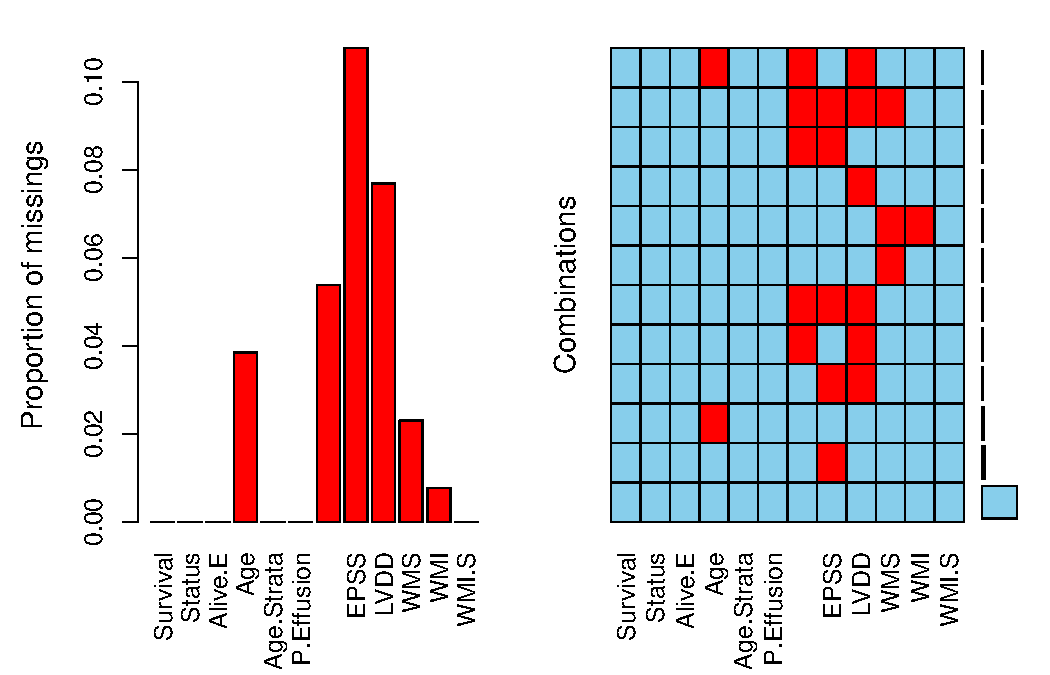
\includegraphics{markdown_files/figure-latex/missing.table-1.pdf}

We leverage the missForest package that uses algorithmic process used
here uses a modified k-nearest neighbor (KNN) approach. Using a training
data set, the routines of the algorithm predicts the missing values
trained on the observed parts of the dataset\textsuperscript{12}. The
process checks each iteration for an acceptable amount of error. If an
iteration produces an error that is smallest than that last iteration,
then the algorithm continues to function. This progress stops when an
error is larger than the previous iteration. Refer to Stekhoven, et. al
2012 for more detail.

We used the missFortune package to run up to 500 iterations. Each
iteration was allotted 1000 trees for the random forest algorithmic
approach.

Following imputation, we verify the imputation accuracy using the
normalized root mean squared error as an indicator of accuracy
(NRMSE)\textsuperscript{8}. The general performance of our imputed
dataset can be expressed by:

\[ NRMSE\ =\ \sqrt{\frac{mean\left(\left(X^{true}-X^{imp}\right)^2\right)}{var\left(X^{true}\right)}} \]

Where X is a matrix of our dataset. Being a random forest iterative
process, each imputed dataset will be different from each other. For our
particular seed and iterations, we obtained a NRMSE value of 0.1442 -
that is our inputted values have an estimate 14.42\% deviation from
estimated true accuracy.

The full imputed dataset may be found in the appendix of this paper. As
well as references to the authors who created the algorithm.

\hypertarget{censoring}{%
\subsubsection{Censoring}\label{censoring}}

Our dataset has numerous censored valued - that is, valued that cannot
be recorded due the constraint of the study design. In our data set, we
are examining the survival after a heart attack, that is, the event of
interest is death given that a patient has had already survived a heart
attack (left truncation).

We have fixed start and end dates for when the data was collection. Some
patients joined when the study began. Others joined later after the
start date. Because of this, we cannot accurately determine how long a
patient survived after our observation period is over. In addition,
there are some patients that have been lost to follow up or may have
died due to the onset of other unrelated factors. These data present
themselves as being randomly right censored.

\hypertarget{methodology}{%
\section{Methodology}\label{methodology}}

Here, we briefly review the methodology and theory behind our analysis
techniques for context.

\hypertarget{non-parametric-kaplan-meier}{%
\subsection{Non-Parametric: Kaplan
Meier}\label{non-parametric-kaplan-meier}}

We use Kaplan-Meier (KM) survival estimators to model a step curve for
the survival of our censored dataset. The KM estimator is an adjustment
of an empirical survival function to reflect the presence of
right-censored observations\textsuperscript{14}. The estimator can be
described in the following equation:

\[ \hat{S}(t) = \prod_{y_{(i)}\leq{t}}^{k} p_i = \prod_{i=1}^{k} (\frac{n_i -d_i}{n_i}) \]

Where \(n_i\) is the number alive before time \(y_i\) and \(d_i\) is the
number of events during during that interval. In our case, \(y_i\) is
the specific patient being observed, \(n_i\) is the number of patients
alive at time \(y_i\). With \(k = 131\), our KM equation is:

\[ \hat{S}(t) = \prod_{i=1}^{131} (\frac{n_i -d_i}{n_i}) \]

We use this equation to estimate the survival at each time interval. We
conduct this analysis for the whole data set and then choose to stratify
on age, pericardial effusion presence, and wall motion score. We also
include cumulative hazard estimators based on the KM fit. Additionally,
as we stratify groups by covariates, we use the Mantel-Haenszel/log-rank
test. The following equation is used to calculate the test statistic in
order to compare two strata\textsuperscript{14}:

\[ Mantel-Haenszel Statistic = \frac
{\sum_{i=1}^{k} (a_i-E_{0}(A_i))}
{\sqrt{\sum_{i=1}^{k} Var_0 (A_i)}}
\]

Where,

\[E_0(A) = \frac{m_1 n_1}{n} \;\; and \;\;\; Var_0(A) =\frac{m_1(n-m_1)}{n-1}*\frac{n_1}{n}(1-\frac{n_1}{n})\]

We then use the Mantel-Haenzel statistics to perform a standard
chi-square test to examine the differences between our strata.

\hypertarget{cumulative-hazard-estimator}{%
\subsubsection{Cumulative Hazard
Estimator}\label{cumulative-hazard-estimator}}

We calculate the hazard of our Kaplan-Survivor function by observing
standard cumulative hazard estimate (shown below):

\[ \hat{H}(t) = -log S(t) = -log \prod_{y_{(i)}\leq{t}} \frac{d_i - n_i}{n_i}  \]

Intuitively, the relationship of the observed hazard is the negative log
of the survival function at each interval. We can clearly see a
graphical relationship between our survival by examining our hazard
plots in the results section. There was the possibility of using
Nelson-Aalen's approximation for hazard, but we find that the
computation is trivial.

\hypertarget{parametric-modeling-of-survival-data}{%
\section{Parametric Modeling of Survival
Data}\label{parametric-modeling-of-survival-data}}

Another technique for characterizing the survival function is to assume
a distributional model for the data. Compared with the Kaplan-Meier
approach, this method has certain advantages that include a continuous
survival curve and simplicity of estimation and prediction. If the
selected model accurately describes the data, it may also lend insight
into the underlying mechanism for the survival behavior. This method is
only applicable if a distributional model can be identified that fits
the survival data adequately.

For the post-myocardial infarction dataset, We fit three commonly
employed distributional models to the survival data and evaluating
goodness of fit of the three models. This is accomplished by comparing
the modeled survival curves to the Kaplan-Meier curve and by comparing
point estimates for each model.

The three models chosen for comparison are the well-known Weibull,
Lognormal, and Loglogistic distributions.

The Weibull hazard function is given below, where \(\lambda\) and
\(\alpha\) are the scale and shape parameters. Weibull hazard is rising
if\(\alpha\) \textgreater{} 1, constant if \(\alpha\) = 1, and declining
if \(\alpha\) \textless{} 1.

\[ \ h(t) = {\lambda}^{-1}{(-log(1-p))}^{1/\alpha} \]

The log-normal distribution can be defined relative to the standard
normal distribution; a random variable Y may be said to have the
log-normal distribution if for some random variable T that has standard
normal distribution:

\[ log (Y) = \alpha + \sigma{T} \]

The hazard function of the log-normal distribution increases with time
from 0 until it reaches a maximum and then decreases, approaching 0 as
time approaches infinity.

The log-logistic distribution can be defined relative to the standard
logistic distribution; a random variable X may be said to have the
log-logistic distribution if for some random variable S that has
standard logistic distribution:

\[ log (X) = \alpha + \sigma{S} \]

the hazard function of the log-logistic distribution decreases with time
from \(\infty\) if \(\alpha\) \textless{} 1, decreases from \(\lambda\)
if \(\alpha\) = 1, and if \(\alpha\) \textgreater{} 1 resembles the
log-normal distribution.

\hypertarget{semi-parametric-modeling-of-survival-data}{%
\section{Semi-Parametric Modeling of Survival
Data}\label{semi-parametric-modeling-of-survival-data}}

Where fully parametric models offer flexibility and the efficient,
relatively simple estimation of overall survival function
parameters,semi-parametric models offer the advantage of being
well-suited to the estimation of covariate effects. Semi-parametric
models decompose risk into a baseline hazard component and a relative
risk component that is dependent on the covariates.

The semi-parametric Cox proportional hazards model is employed here to
explore the relationship between predictor variables and survival
behavior.

The Cox PH hazard function is defined as follows:

\[ h(t)=h_0(t)×exp(b_1x_1+b_2x_2+...+b_nx_n) \]

where t represents the survival time, \(x_1,x_2,...,x_n\) are the set of
prognostic factors or covariates, and the coefficients
\(b_1,b_2,...,b_n\) measure the effect of the covariates on survival
time. The baseline hazard \(h_0(t)\) corresponds to the value of the
hazard if all covariates are equal to zero.

Use of the Cox PH model requires that the baseline hazard is not
dependent on the covariates, and that the covariate terms do not depend
on time - that is, that the slope coefficients are constant. Hazard
functions stratified on covariate group may be used to assess the
proportional hazard assumption. If the hazards functions for covariate
groups cross over time, the proportionality assumption is not met and
alternate analysis methods should be employed. One such method involves
sub-setting the survival data and covariates based on hazard cross-over
time. In this approach, a separate model is fit to each subset where it
has been determined that the proportionality assumption holds.
Alternately one may apply alternate modeling techniques that are
suitable for time-varying effects, or simply investigate the impact of
covariate by inspection of stratified Kaplan-Meier survival curves (Kim,
2000).

\hypertarget{results}{%
\section{Results}\label{results}}

\hypertarget{non-parametric-kaplan-meier-survival-estimates}{%
\subsection{Non-Parametric: Kaplan-Meier Survival
Estimates}\label{non-parametric-kaplan-meier-survival-estimates}}

Kaplan-Meier estimates give us the following curve (full KM estimator
table can be found in the appendix).

\begin{center}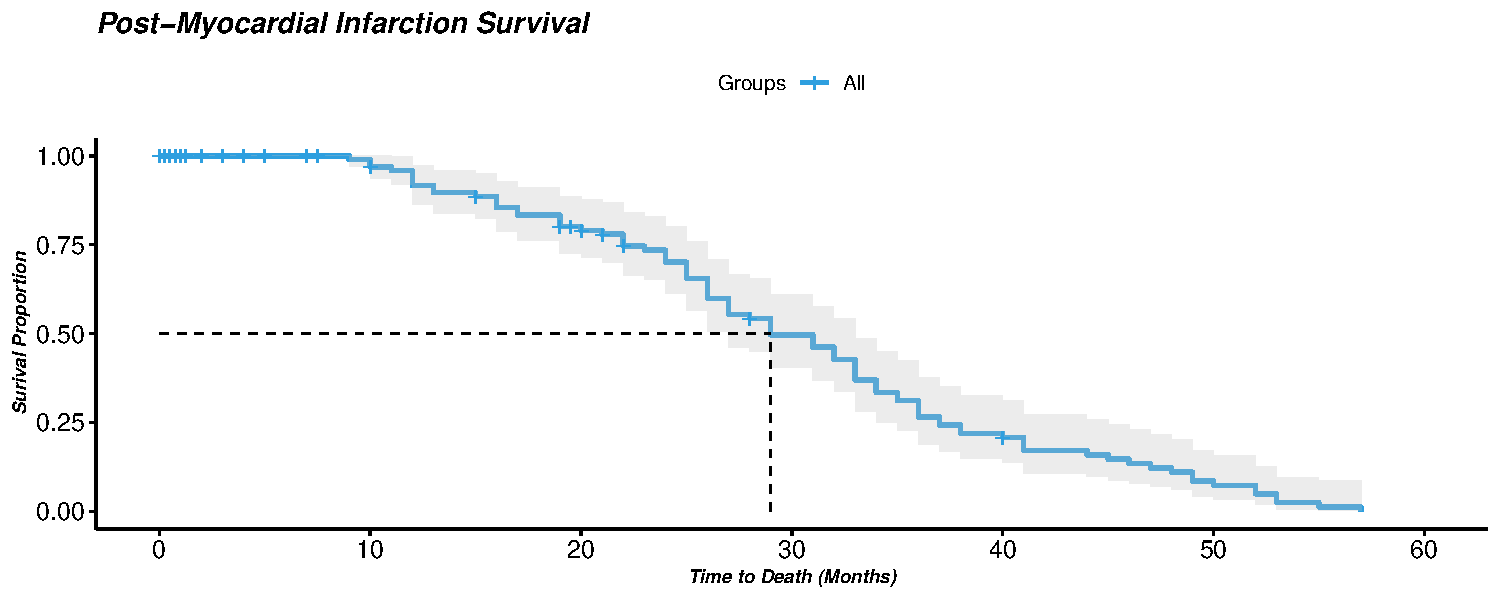
\includegraphics{markdown_files/figure-latex/km.all-1} \end{center}

\begin{table}[!h]

\caption{\label{tab:ks1}Kaplan-Meier Estimates for All Groups}
\centering
\begin{tabular}[t]{l|c|c|c|c|c|c}
\hline
  & Records & Events & Mean & Median & Median 0.95 LCL & Median 0.95 UCL\\
\hline
All Groups & 130 & 88 & 30.53 & 29 & 27 & 33\\
\hline
\end{tabular}
\end{table}

The Kaplan-Meier estimates for for all groups within our dataset is
shown above. The curve follows a general pattern of decreasing
survivability over time. With time spanning to a maximum of 57 months,
we have a mean survival time of approximately 30.5 months. The median
survival time is 29 months with 95\% confidence limits between 27 and 33
months.

When testing for significant difference between strata groups we use the
log-ran

\begin{center}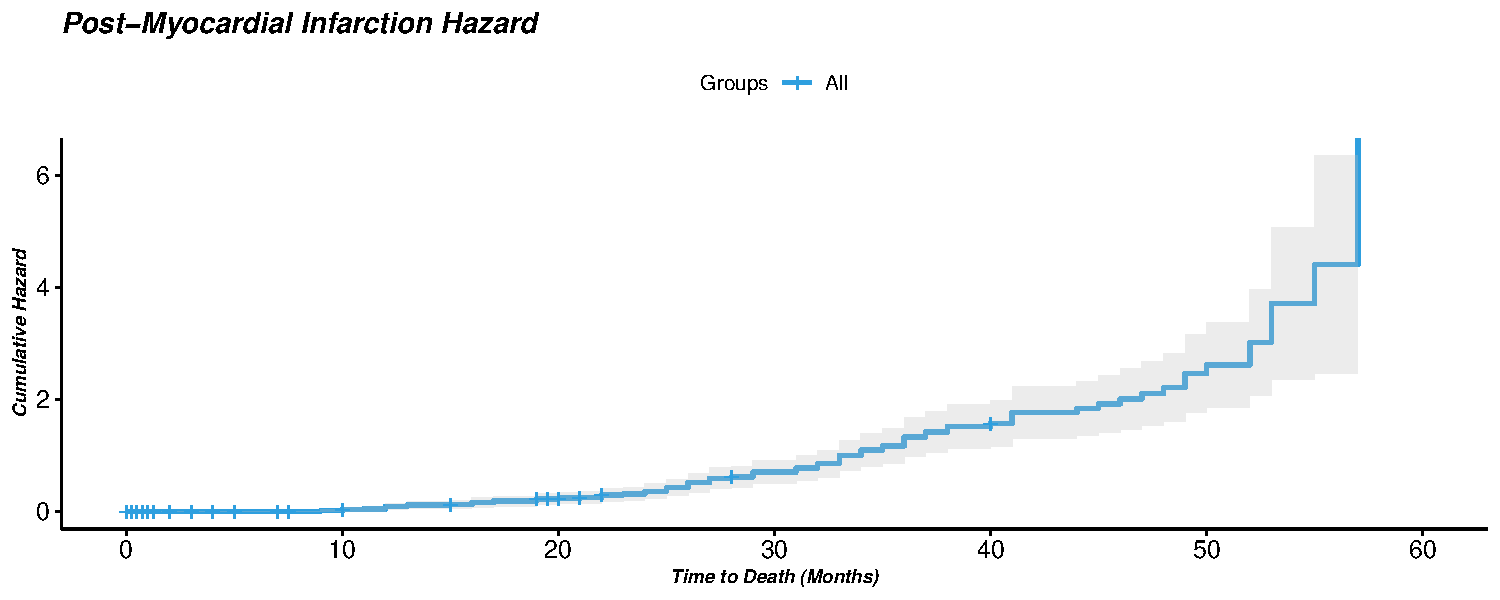
\includegraphics{markdown_files/figure-latex/kmhaz.all-1} \end{center}

To explore differences among groups, we stratify among age, pericardial
effusion presence, wall motion score, and fractional shortening. We
first begin exploring the effects of age and pericardial effusion
presence:

\hypertarget{stratified-by-age-and-pericardial-effusion-presence}{%
\subsubsection{Stratified by Age and Pericardial Effusion
Presence}\label{stratified-by-age-and-pericardial-effusion-presence}}

The results of a Kaplan-Meier estimate for age and pericardial effusion
stratification can be seen below:

\begin{center}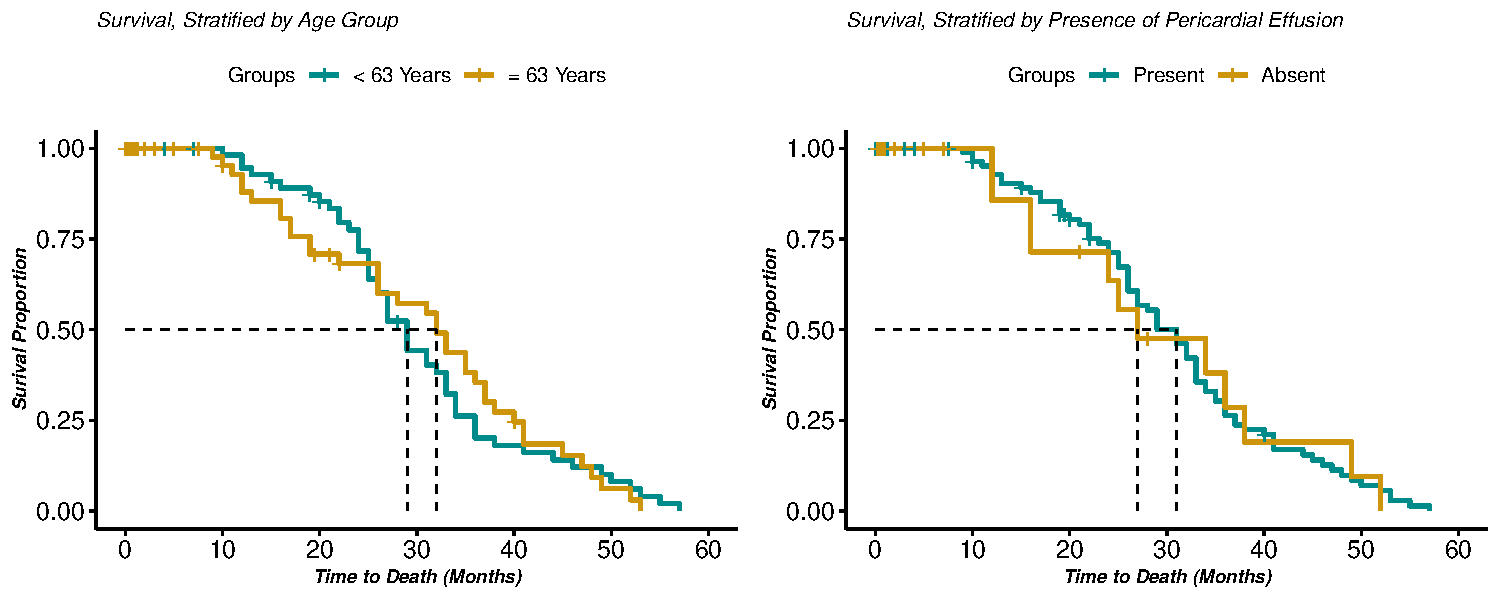
\includegraphics{markdown_files/figure-latex/km.age.effusion-1} \end{center}

\begin{table}[!h]

\caption{\label{tab:ks2}Kaplan-Meier Estimates Stratified by Age and Pericardial Effusion Presence}
\centering
\begin{tabular}[t]{l|c|c|c|c|c|c}
\hline
  & Records & Events & Mean & Median & Median 0.95 LCL & Median 0.95 UCL\\
\hline
Age < 63 & 66 & 51 & 30.47 & 29 & 26 & 33\\
\hline
Age = 63 & 64 & 37 & 30.60 & 32 & 26 & 37\\
\hline
Absent & 106 & 76 & 30.63 & 31 & 27 & 33\\
\hline
Present & 24 & 12 & 29.94 & 27 & 24 & NA\\
\hline
\end{tabular}
\end{table}

\begin{table}

\caption{\label{tab:ks2.survdiff}Summary of Differences Between Strata}
\centering
\begin{tabular}[t]{l|r|r|r}
\hline
  & N & Observed & Expected\\
\hline
Age < 63 & 66 & 51 & 50.58084\\
\hline
Age ≥ 63 & 64 & 37 & 37.41916\\
\hline
Absent & 106 & 76 & 76.42260\\
\hline
Present & 24 & 12 & 11.57740\\
\hline
\end{tabular}
\end{table}

When stratified by age, we find a slight difference between the curves.
The age group younger than 63 has a mean survival time of 30.47 months
with a median survival time of 29 months. The older group - ages greater
than 63 - has a similar mean survival time of 30.6 months and a slightly
longer median survival time of 32 months. When comparing the presence of
pericardial effusion, there are 106 cases where the effusion is absent,
while 24 cases have the effusion present. The mean survival time when
pericardial effusion is absent is 30.63 months with a median survival
time of 31 months. For converse case, the mean survival time is 29.94
months while the median is lower at 27 months.

\begin{center}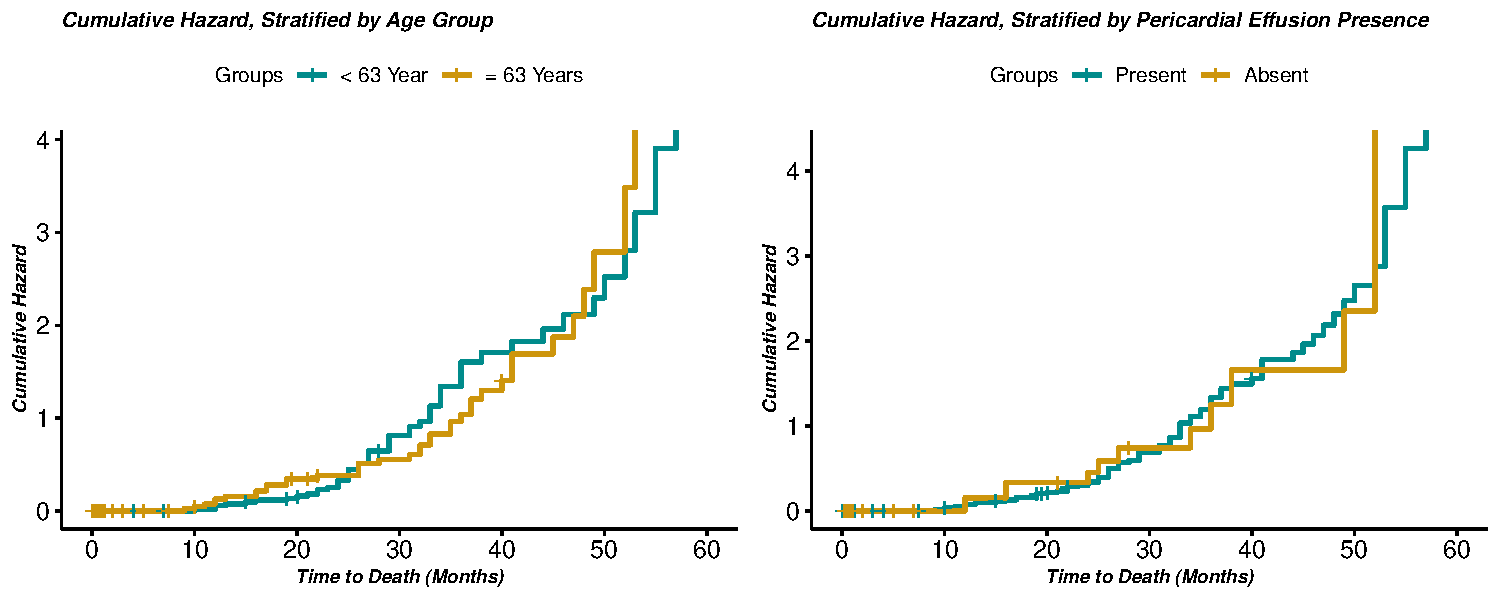
\includegraphics{markdown_files/figure-latex/km.haz1-1} \end{center}

For both groups, there does not seem to be a large departure from
cumulative hazard. When stratifying by age, we see a slight increase in
cumulative hazard of the younger group between 30 and 50 months. After
that mark, the older group experiences a relative increase in cumulative
hazard. When stratified by pericardial effusion presence, very little
difference can be observed with any difference being the result of
sample size differences.

\hypertarget{stratified-by-wall-motion-score-and-fractional-shortening-length}{%
\subsubsection{Stratified by Wall Motion Score and fractional Shortening
Length:}\label{stratified-by-wall-motion-score-and-fractional-shortening-length}}

We then explore the effects of wall motion score and fractional
shortening:

\begin{center}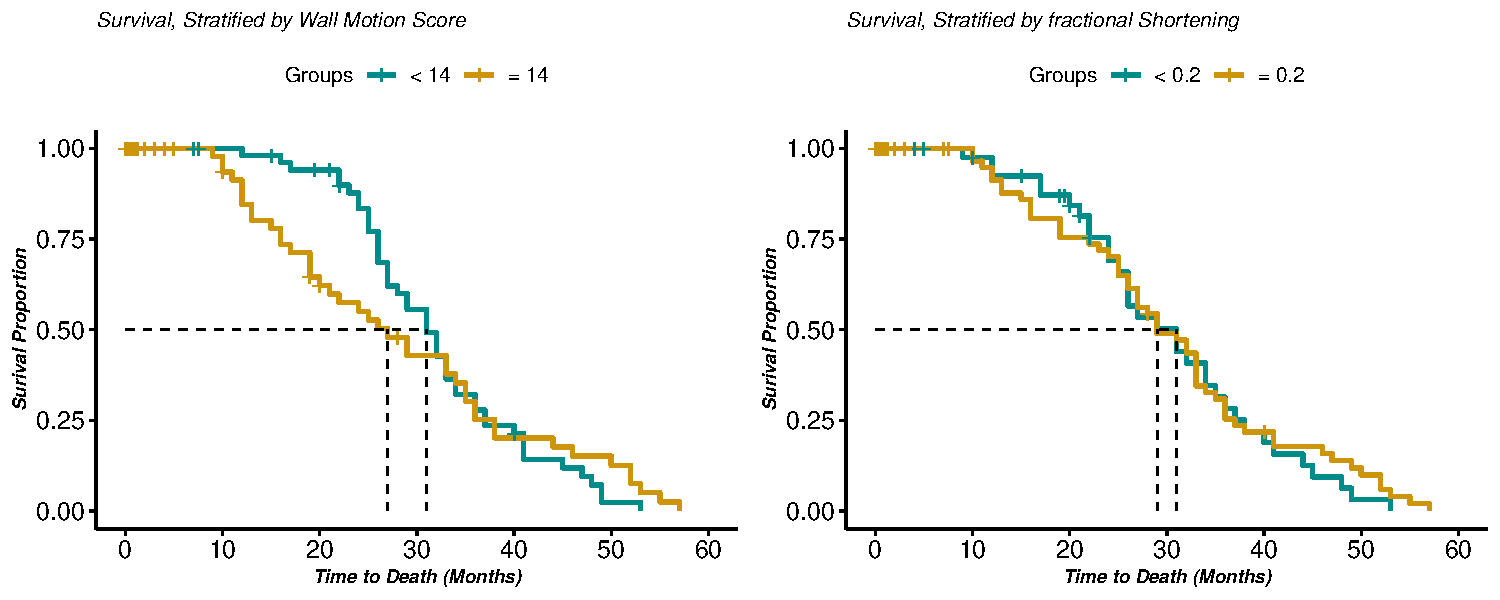
\includegraphics{markdown_files/figure-latex/km.wms.fshort-1} \end{center}

\begin{table}[!h]

\caption{\label{tab:ks4}Kaplan-Meier Estimates Stratified by Wall Motion Score and fractional Shortening}
\centering
\begin{tabular}[t]{l|c|c|c|c|c|c}
\hline
  & Records & Events & Mean & Median & Median 0.95 LCL & Median 0.95 UCL\\
\hline
Score < 14 & 62 & 46 & 32.17 & 31 & 27 & 34\\
\hline
Score = 14 & 68 & 42 & 28.61 & 27 & 20 & 35\\
\hline
Length < 0.2 & 61 & 33 & 30.45 & 31 & 26 & 36\\
\hline
Length = 0.2 & 69 & 55 & 30.44 & 29 & 26 & 33\\
\hline
\end{tabular}
\end{table}

\begin{table}

\caption{\label{tab:ks4.5.survdiff}Summary of Differences Between Strata}
\centering
\begin{tabular}[t]{l|r|r|r}
\hline
  & N & Observed & Expected\\
\hline
Wall Motion Score < 14 & 66 & 51 & 50.58084\\
\hline
Wall Motion Score ≥ 14 & 64 & 37 & 37.41916\\
\hline
Fractional Shortening < 0.2 & 106 & 76 & 76.42260\\
\hline
Fractional Shortening ≥ 0.2 & 24 & 12 & 11.57740\\
\hline
\end{tabular}
\end{table}

\begin{verbatim}

When stratified by wall motion score, we find a difference between the curves. Wall motion scores less than 14 have a mean survival time of 32.17 months with a median survival time of 31 months. Wall motion scores greater or equal to 14 have a lower mean survival time of 28.61 months and a median survival time of 27 months.

When stratified by fractional shortening length, both groups have a similar mean at approximately 30.4 months. When fractional shortening is less than 0.2, the median survival time is 31 months while having a fractional shortening length that is greater than 0.2, we have a slightly lower median survival time of 29 months.


\begin{center}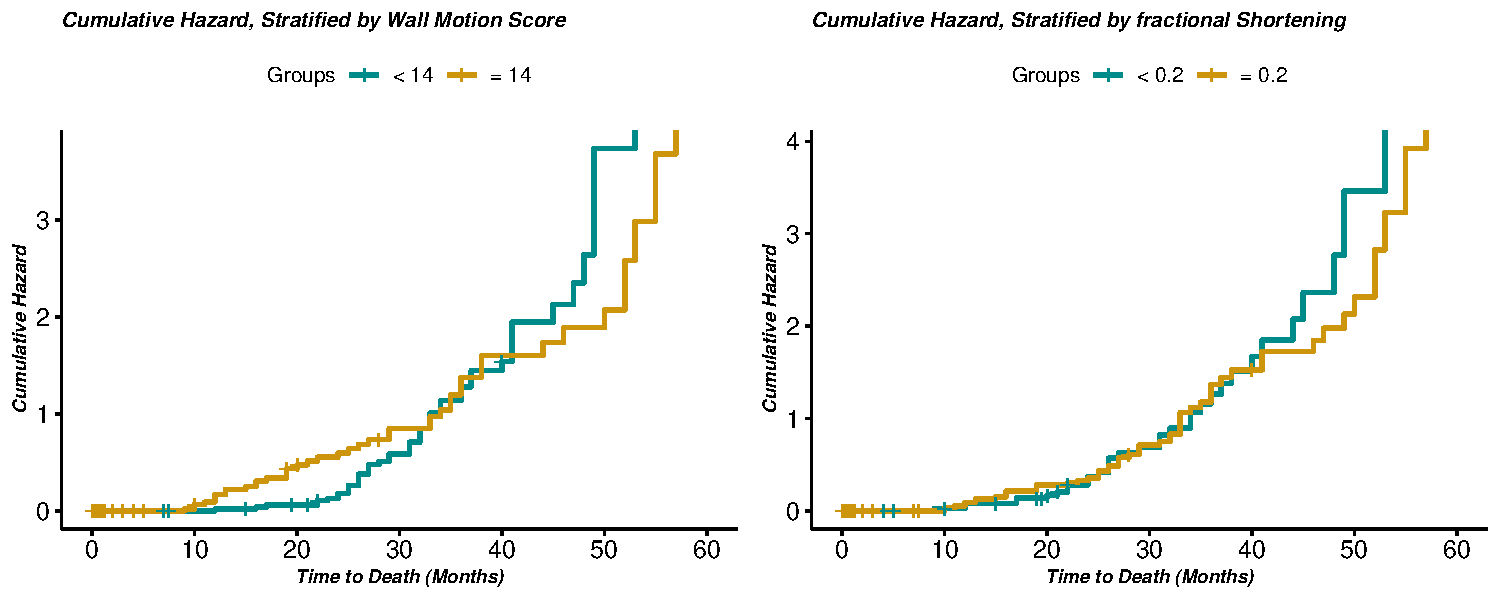
\includegraphics{markdown_files/figure-latex/km.haz2-1} \end{center}

Here, we see some minute differences between the hazard curves. When stratified by Wall Motion Score, we see some overlap in the initial stages of the study as well as around approximately 35 months. The exceptions are seen with higher wall motion scores seeing increased risk before the median and decreased relative risk after the median. The converse is seen for the lower wall motion scores.

When stratified by fractral shortening, the cumulative hazard curves are approximately similar with higher fractional shortening lengths have less risk after the median.

## Parameter Estimation

The estimated distributional model curves are overlaid on the K-M curve for the post-myocardial infarction data in the figures below. 


\begin{center}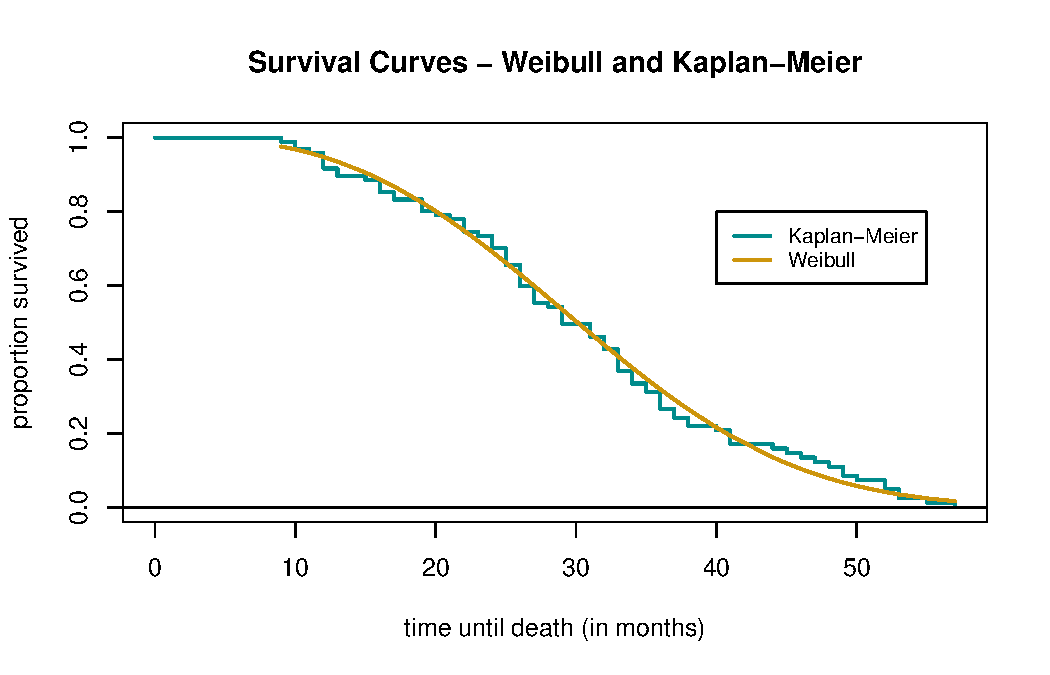
\includegraphics{markdown_files/figure-latex/unnamed-chunk-1-1} \end{center}



\begin{center}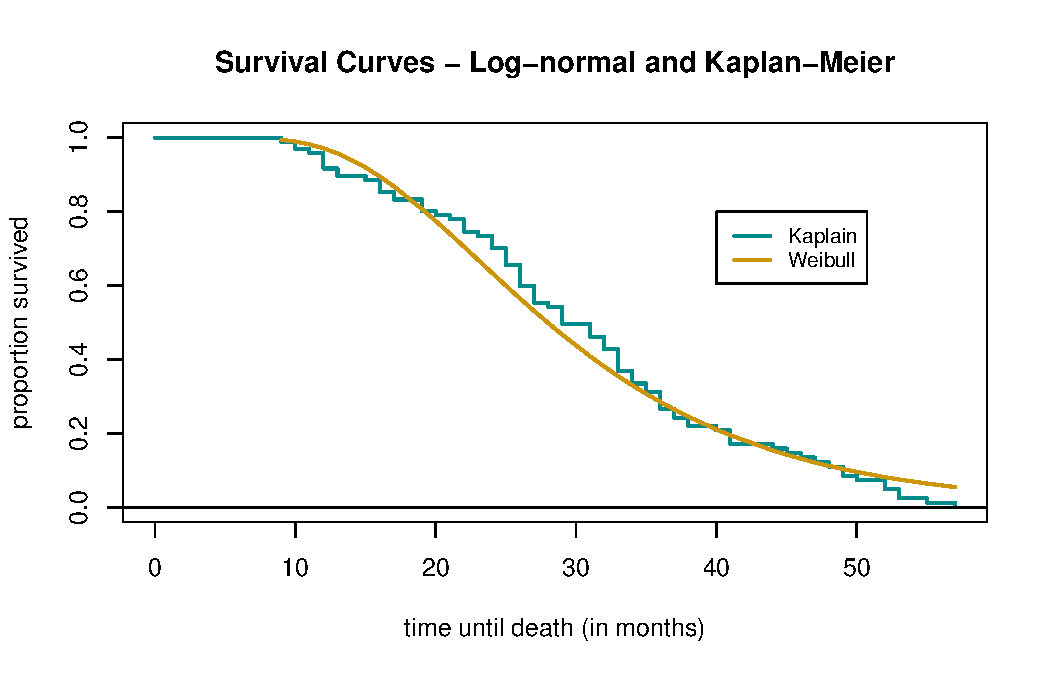
\includegraphics{markdown_files/figure-latex/unnamed-chunk-1-2} \end{center}



\begin{center}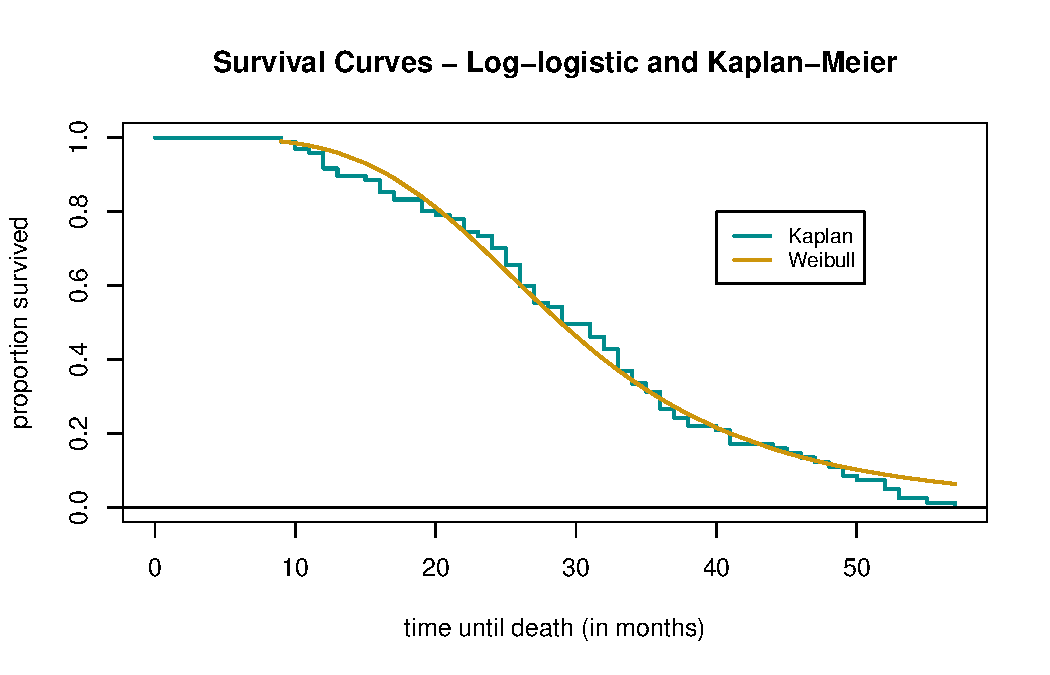
\includegraphics{markdown_files/figure-latex/unnamed-chunk-1-3} \end{center}



The table below summarizes the parameter point estimates and corresponding 95% confidence intervals. 



\begin{tabular}{l|r|r|r|r|r}
\hline
Model & Quantile & Point Estimate & 95\% LCL & 95\% UCL & Interval Length\\
\hline
Weibull & 0.25 & 22.42 & 19.96 & 25.19 & 5.23\\
\hline
NA & 0.50 & 30.32 & 27.86 & 33.01 & 5.15\\
\hline
NA & 0.75 & 38.47 & 35.71 & 41.44 & 5.72\\
\hline
Log-normal & 0.25 & 20.73 & 18.77 & 22.89 & 4.11\\
\hline
NA & 0.50 & 27.97 & 25.54 & 30.63 & 5.09\\
\hline
NA & 0.75 & 37.74 & 34.06 & 41.83 & 7.77\\
\hline
Log-logistic & 0.25 & 21.90 & 19.77 & 24.27 & 4.50\\
\hline
NA & 0.50 & 28.88 & 26.41 & 31.59 & 5.18\\
\hline
NA & 0.75 & 38.09 & 34.45 & 42.12 & 7.67\\
\hline
\end{tabular}


Q-Q plots were also prepared for each distribution, and are provided in the Appendix. Based on inspection of the Q-Q plots and the K-M overlay plots, we found that the Weibull model appears to provide the best fit. In addition, it was noted that the confidence intervals for point estimation were overall more narrow for the Weibull model compared to log-normal and log-logistic. It was also observed that the point estimate for median is close to that identified by the Kaplan-Meier approach (29 months in K-M estimation, 30 months when estimating with Weibull fit). We propose the Weibull model as descriptive of the post-myocardial infarction survival data.

## Regression Analysis - Cox Proportional Hazard Modeling 

Regression analysis was conducted to identify the relationship between potential predictor variables and survival. As a first step, the covariate pool was screened for potential multicolinearity (see Appendix for plots of the covariates). Potential dependency was observed between Fractional Shortening, E-Point Septal Separation, and Left Ventrical Diastolic Dysfunction. Mechanistically, this is intuitive, since all three variables measure ventrical diastolic behavior. Models were fit with each of these colinear variables, and based on this assessment of Fractional Shortening was selected for inclusion in the final covariate pool of potential prognostic factors for regression. These covariates are:  

\begin{description}
  \item[$\bullet$] Age
  \item[$\bullet$] Pericardial Effusion
  \item[$\bullet$] Wall Motion Score
  \item[$\bullet$] Fractional Shortening
\end{description}

A model employing all of the covariates listed above was created. In order to test validit of the proportional hazard assumption, survival curves stratified by group were assessed for each of the four selected covariates. It was found that the proportional hazard assumption does not hold, as hazards for each group cross over with time for each covariate. 

This limitation was addressed through the identification of survival time subsets in which covariates met the proportional hazards assumption, and could thus be employed as predictor variables. These subsets were identified by inspecting hazard function data stratified on all covariates and identifying regions of crossover. (See Appendix for plots of stratified hazard functions with the approximate crossover regions marked).

The selected time subsets were obtained as follows:

\begin{description}
 \item[$Subset \:1: t \leq {26} \:{months}$]
 \item[$Subset \:2:26 \:{months}< t < 46 \:{months}$]
 \item[$Subset \:3: 46 \: months \leq t$]
\end{description}

Within each time subset, the proportional hazard assumption was tested for each of the four covariates and found to hold. A Cox PH model was fitted to each subset of the survival data, reduced as far as possible using a Step AIC procedure with Likelihood Ratio Test selection, and evaluated for adequacy using standard diagnostic techniques. 

The three models are summarized below: 


\begin{tabular}{l|l|l|l|l|l|l|l|l|l}
\hline
**Characteristic** & **HR** & **95\% CI** & **p-value** & **HR** & **95\% CI** & **p-value** & **HR** & **95\% CI** & **p-value**\\
\hline
Wall\_Motion\_Score & 0.85 & 0.69, 1.05 & 0.13 & 0.90 & 0.79, 1.02 & 0.11 &  &  & \\
\hline
Fractional\_Shortening & 0.00 & 0.00, 0.01 & 0.009 &  &  &  &  &  & \\
\hline
Wall\_Motion\_Score * Fractional\_Shortening & 4.31 & 1.51, 12.4 & 0.006 &  &  &  &  &  & \\
\hline
Age &  &  &  &  &  &  & 0.96 & 0.92, 1.00 & 0.051\\
\hline
\end{tabular}
For Model 1, the significant predictors of survival time are identified as Fractional Shortening and its interaction with Wall Motion Score. Although Wall Motion Score does not have a significant effect on survival as a main effect, it is retained due to is presence in the interaction term.  

For Model 2, the significant predictor of survival time is identified as patient age. Age is found to have a very weak effect on survival; none of the echocardiographic covariates had an impact on survival in this time region. Both these findings are supported by inspection of the stratified hazard function plots.  

For subset 3, the sample size of events in the survival data subset was small (n=11) and a significant model was not obtained. The model is presented for context but is poorly descriptive of the relationship between prognostic factors and survival.

Model residual diagnostics were assessed for all three models. Models 1 and 2 showed overall good fit to the data and demonstrated proportional hazard assumption compliance. As expected given the discussion above, Model 3 did not result in a good overall fit, although proportional hazard assumption was met. Model diagnostic residual plots and further discussion may be found in the Appendix. 

# Discussion

## Explanation of results
In our non-parametric analysis, median survival times for nearly all of the stratification elements show relatively similar results with the exception of high wall motion scores. When stratified by age group, we see relatively similar survival proportions with some distinction before and after the median. Before the median, the older group has a slightly lower survival proportion. However, after the median, the older group has a slightly higher survival proportion before 45 months. This slight discrepancy could be due to the externalities attached to young heart attack patients. If patients are experiencing heart attacks at a younger age, there could be higher chances that those patients already have other health concerns. Patients experiencing and surviving a heart attack at older ages could be in physically superior condition than their younger counterparts. All other stratification groups show relatively similar median survival proportions. An interesting observation can be seen when we arbitrarily divide the age strata into three groups. We see a much greater risk associated with patients younger than 55 while all other age groups perform similarly.

In the parametric analysis, it was found that the survivor data is well-described by the Weibull distribution. This finding enables the construction of a continuous survivor function and provides the opportunity for flexible point estimation as well as estimation of survival probability over a given input time. Semi-parametric modeling was also performed. Three Cox Proportional Hazards models were developed that described the relationship between prognostic factors and survival; one for short survival times; one for intermediate survival times; and another for long survival times. Given a small sample size for long survival times, only the first two models were significant. A key finding from this analysis is that when survival time is shorter, abnormalities in the echocardiographic profile of the patient's heart are what predict survival, rather than age. Conversely, when the survival times are longer, it is the age of the patient that predicts survival (albeit weakly), rather than any of the echocardiographic properties do not. This is consistent with the behavior of the stratified hazard curves for these variables over time. This result seems to imply that in the acute recovery period following a myocardial infarction, patient prognosis is closely tied to heart health; but as time progresses, patient age becomes the key driver of prognosis. This finding is intuitive, since as treatment and recovery progress over time, risk related to the myocardial event would decrease and other pre-existing risks would play a larger role in survival. 

## Summary of Limitations
Very clearly, our data is smaller than we hoped for, both in the number of observations and in the availability of meaningful prognostic factors. Development of a single large regression fit that reliably predicts covariates would require a much larger dataset. In particular, the lack of gender as an available covariate is a potential limitation of our data, as the effect of gender on heart-related survival is well established in the literature. Longer collection period over a greater number of patients would yield stronger regression model development. As-is, there is not enough data to produce a significant model across the entire survival time window. 

A particular limitation related to subgroup dimension was identified through the stratification analysis. Examination of stratified data showed relative unequal distributions among groups. For example, when examining pericardial effusion, we compare 106 records of with effusion absent to 24 records of effusion present. Given that the collection methods are unclear and the groups sizes are so much different form each other, we cannot fully be confident in our results. Such comparisons are unequal comparisons. 

Finally, the given dataset did not have clear statements as to what data collection methods were used. Given our smaller sample size and these unknown methods, we cannot be entirely confident that our results reflect the survival behavior of the population as a whole. Future studies would benefit greatly 

## Conclusion
This study identified a variety of properties of the post-myocardial infarction survival data. The overall survival function was characterized by both non-parametric Kaplan-Meier and Weibull models, and point estimates determined. Analysis of the effect of echocardiographic data and of age on survival was performed both by inspection of stratified survival curves and by regression analysis. Findings included that age group has an impact on survival, but that this effect potentially varies over time, and that certain heart-related prognostic factors (in particular wall motion score and its interaction with fractional shortening) also have an impact on survival that varies over time. We conclude that future studies should expand on collection of variables that could potentially influence survivability, as well as the cohort size and length of follow-up period. Interesting effects to include may include poverty, diet, ethnicity, race, sex, and even work place stress/effects. Finally, further investigation with a larger dataset on the relationship between acute survival time and echocardiographic data profile and between the relationship of age group on survival data  may yield useful insights into specific risk profiles for post-myocardial infarction patients. 

\newpage

# Appendix

## References

1. Andrikopoulos, G. K., Tzeis, S. E., Pipilis, A. G., Richter, D. J., Kappos, K. G., Stefanadis, C. I., … Chimonas, E. T. (2006). Younger age potentiates post myocardial infarction survival disadvantage of women. International Journal of Cardiology, 108(3), 320–325. doi: 10.1016/j.ijcard.2005.05.016

2. Fryar CD, Chen T-C, Li X. Prevalence of uncontrolled risk factors for cardiovascular disease: United States, 1999–2010 pdf icon[PDF-494K]. NCHS data brief, no. 103. Hyattsville, MD: National Center for Health Statistics; 2012. Accessed May 9, 2019.

3. Ford, E. S., & Capewell, S. (2007). Coronary Heart Disease Mortality Among Young Adults in the U.S. From 1980 Through 2002. Journal of the American College of Cardiology, 50(22), 2128–2132. doi: 10.1016/j.jacc.2007.05.056

4. Dalen JE, Alpert JS, Goldberg RJ, Weinstein RS. The epidemic of the 20(th) century: coronary heart disease. Am J Med. 2014;127(9):807‐812. doi:10.1016/j.amjmed.2014.04.015

5. Goldman, L. (1984). The Decline in Ischemic Heart Disease Mortality Rates. Annals of Internal Medicine, 101(6), 825. doi: 10.7326/0003-4819-101-6-825

6. Gu K, Cowie CC, Harris MI. Diabetes and Decline in Heart Disease Mortality in US Adults. JAMA. 1999;281(14):1291–1297. doi:10.1001/jama.281.14.1291

7. Heron, M. Deaths: Leading causes for 2017 pdf icon[PDF – 3 M]. National Vital Statistics Reports;68(6). Accessed November 19, 2019.

8. Kan, G., Visser, C., Kooler, J., & Dunning, A. (1986). Short and long term predictive value of wall motion score in acute myocardial infarction. British Heart Journal, 56, 422-427.

9. Oba S, Sato MA, Takemasa I, Monden M, Matsubara K, Ishii S. A Bayesian missing value estimation method for gene expression profile data. Bioinformatics. 2003;19(16):2088‐2096. doi:10.1093/bioinformatics/btg287

10. Rimm, E. B., Stampfer, M. J., Giovannucci, E., Ascherio, A., Spiegelman, D., Colditz, G. A., & Willett, W. C. (1995). Body Size and Fat Distribution as Predictors of Coronary Heart Disease among Middle-aged and Older US Men. American Journal of Epidemiology, 141(12), 1117–1127. doi: 10.1093/oxfordjournals.aje.a117385 

11. Salzberg, S. (1988). Exemplar-based learning: Theory and implementation (Technical Report TR-10-88). Harvard University, Center for Research in Computing Technology, Aiken Computation Laboratory (33 Oxford Street; Cambridge, MA 02138).

12. Sia, Y. T., Parker, T. G., Liu, P., Tsoporis, J. N., Adam, A., & Rouleau, J. L. (2002). Improved post-myocardial infarction survival with probucol in rats: Effects on left ventricular function, morphology, cardiac oxidative stress and cytokine expression. Journal of the American College of Cardiology, 39(1), 148–156. doi: 10.1016/s0735-1097(01)01709-0

13. Stekhoven, D. J., & Buhlmann, P. (2011). MissForest--non-parametric missing value imputation for mixed-type data. Bioinformatics, 28(1), 112–118. doi: 10.1093/bioinformatics/btr597 

14. Tableman, M., & Kim, J. S. (2004). Survival analysis using S: analysis of time-to-event data. Boca Raton, Florida: Chapman & Hall.

15. Wilmot, K. A., O’Flaherty, M., Capewell, S., Ford, E. S., & Vaccarino, V. (2015). Coronary Heart Disease Mortality Declines in the United States From 1979 Through 2011CLINICAL PERSPECTIVE. Circulation, 132(11), 997–1002. doi: 10.1161/circulationaha.115.015293


\newpage


## Dataset Variable Summary


\begin{longtabu} to \linewidth {>{\raggedright}X>{\raggedright}X>{\raggedright}X}
\caption{\label{tab:Dataset.summary}Summary of Dataset Covariates}\\
\toprule
Variable & Label & Definition\\
\midrule
\endfirsthead
\caption[]{Summary of Dataset Covariates \textit{(continued)}}\\
\toprule
Variable & Label & Definition\\
\midrule
\endhead
\
\endfoot
\bottomrule
\endlastfoot
Survival & Survival & The number of months the patints survived, post-myocardial infarction.\\
\addlinespace
Status & Status & Censorship status. 0 denotes that a patient is a censored while 1 denotes that a patient is uncensored.\\
\addlinespace
Alive at the end of Survival Period & Alive.E & Binary variable. 0 denotes that patient is alive at the end of the survival period while 1 indicates that a patient is still alive.\\
\addlinespace
Patient Age & Age & The age in years when a myocardial infarction occurs.\\
\addlinespace
Age Group & Age.S & 0 denotes younger than 55 years . 1 denotes 55 - 70 years. 2 denotes older than 70\\
\addlinespace
Pericardial Effusion & P.Effusion & Binary variable. Pericardial effusion is excess fluid surrounding the heart. Though excess is not harmful, it is sometimes indicates a porly functioning heart. 0 denotes that pericardial effusion is absent while 1 denotes that fluid is present.\\
\addlinespace
Fractional Shortening & F.Shortening & Fractional shortening is a measure of contractility around the heart. Generally, lower numbers are considered to be abnormal.\\
\addlinespace
E-Point Septal Separation & EPSS & E-point septal separation is an addition measure of heart contractivity. Larger numbers are considered to be abnormal.\\
\addlinespace
Left Ventricular End-Diastolic Dimension & LVDD & Left ventricular end-diastolic dimension is the measure of the heart at the end of disatole. The larger this value is indicates a larger heart. Larger hearts are generally in poor health.\\
\addlinespace
Wall Motion Score & WMS & Wall motion score is a measure of how the segments of the left ventricle are moving during systol.\\
\addlinespace
Wall Motion Index & WMI & Wall motion index is the wall motion score divided by the number of segments that are moving. Normally, 12-13 segments can be seen in an echocardiogram.\\
\addlinespace
Wall Motion Strata & WMS.S & 0 denotes score less than 11, 1 denotes score 12-14, 2 denotes score greater than 14\\*
\end{longtabu}


## Original Dataset


\begin{longtabu} to \linewidth {>{\raggedleft}X>{\raggedleft}X>{\raggedleft}X>{\raggedleft}X>{\raggedleft}X>{\raggedleft}X>{\raggedleft}X>{\raggedleft}X>{\raggedleft}X>{\raggedleft}X>{\raggedleft}X>{\raggedleft}X}
\caption{\label{tab:Dataset.actual}Original Dataset}\\
\toprule
Survival & Status & Alive.E & Age & Age.Strata & P.Effusion & F.Shortening & EPSS & LVDD & WMS & WMI & WMI.S\\
\midrule
\endfirsthead
\caption[]{Original Dataset \textit{(continued)}}\\
\toprule
Survival & Status & Alive.E & Age & Age.Strata & P.Effusion & F.Shortening & EPSS & LVDD & WMS & WMI & WMI.S\\
\midrule
\endhead
\
\endfoot
\bottomrule
\endlastfoot
11.00 & 1 & 0 & 71.00 & 2 & 0 & 0.260 & 9.000 & 4.600 & 14.00 & 1.000 & 0\\
19.00 & 1 & 0 & 72.00 & 2 & 0 & 0.380 & 6.000 & 4.100 & 14.00 & 1.700 & 1\\
16.00 & 1 & 0 & 55.00 & 1 & 0 & 0.260 & 4.000 & 3.420 & 14.00 & 1.000 & 0\\
57.00 & 1 & 0 & 60.00 & 1 & 0 & 0.253 & 12.062 & 4.603 & 16.00 & 1.450 & 1\\
19.00 & 0 & 1 & 57.00 & 1 & 0 & 0.160 & 22.000 & 5.750 & 18.00 & 2.250 & 1\\
\addlinespace
26.00 & 1 & 0 & 68.00 & 2 & 0 & 0.260 & 5.000 & 4.310 & 12.00 & 1.000 & 0\\
13.00 & 1 & 0 & 62.00 & 1 & 0 & 0.230 & 31.000 & 5.430 & 22.50 & 1.875 & 1\\
50.00 & 1 & 0 & 60.00 & 1 & 0 & 0.330 & 8.000 & 5.250 & 14.00 & 1.000 & 0\\
19.00 & 1 & 0 & 46.00 & 0 & 0 & 0.340 & 0.000 & 5.090 & 16.00 & 1.140 & 0\\
25.00 & 1 & 0 & 54.00 & 1 & 0 & 0.140 & 13.000 & 4.490 & 15.50 & 1.190 & 0\\
\addlinespace
10.00 & 0 & 1 & 77.00 & 2 & 0 & 0.130 & 16.000 & 4.230 & 18.00 & 1.800 & 1\\
52.00 & 1 & 0 & 62.00 & 1 & 1 & 0.450 & 9.000 & 3.600 & 16.00 & 1.140 & 0\\
52.00 & 1 & 0 & 73.00 & 2 & 0 & 0.330 & 6.000 & 4.000 & 14.00 & 1.000 & 0\\
44.00 & 1 & 0 & 60.00 & 1 & 0 & 0.150 & 10.000 & 3.730 & 14.00 & 1.000 & 0\\
0.50 & 0 & 1 & 62.00 & 1 & 0 & 0.120 & 23.000 & 5.800 & 11.67 & 2.330 & 1\\
\addlinespace
24.00 & 1 & 0 & 55.00 & 1 & 1 & 0.250 & 12.063 & 4.290 & 14.00 & 1.000 & 0\\
0.50 & 0 & 1 & 69.00 & 2 & 1 & 0.260 & 11.000 & 4.650 & 18.00 & 1.640 & 1\\
0.50 & 0 & 1 & 62.53 & 1 & 1 & 0.070 & 20.000 & 5.200 & 24.00 & 2.000 & 1\\
22.00 & 0 & 1 & 66.00 & 2 & 0 & 0.090 & 17.000 & 5.819 & 8.00 & 1.333 & 1\\
1.00 & 0 & 1 & 66.00 & 2 & 1 & 0.220 & 15.000 & 5.400 & 27.00 & 2.250 & 1\\
\addlinespace
0.75 & 0 & 1 & 69.00 & 2 & 0 & 0.150 & 12.000 & 5.390 & 19.50 & 1.625 & 1\\
0.75 & 0 & 1 & 85.00 & 2 & 1 & 0.180 & 19.000 & 5.460 & 13.83 & 1.380 & 1\\
0.50 & 0 & 1 & 73.00 & 2 & 0 & 0.230 & 12.733 & 6.060 & 7.50 & 1.500 & 1\\
5.00 & 0 & 1 & 71.00 & 2 & 0 & 0.170 & 0.000 & 4.650 & 8.00 & 1.000 & 0\\
48.00 & 1 & 0 & 64.00 & 1 & 0 & 0.190 & 5.900 & 3.480 & 10.00 & 1.110 & 0\\
\addlinespace
29.00 & 1 & 0 & 54.00 & 1 & 0 & 0.300 & 7.000 & 3.850 & 10.00 & 1.667 & 1\\
29.00 & 1 & 0 & 35.00 & 0 & 0 & 0.300 & 5.000 & 4.170 & 14.00 & 1.000 & 0\\
29.00 & 1 & 0 & 55.00 & 1 & 0 & NA & 7.000 & NA & 2.00 & 1.000 & 0\\
0.25 & 0 & 1 & 75.00 & 2 & 0 & NA & NA & NA & NA & 1.000 & 0\\
36.00 & 1 & 0 & 55.00 & 1 & 1 & 0.210 & 4.200 & 4.160 & 14.00 & 1.560 & 1\\
\addlinespace
1.00 & 0 & 1 & 65.00 & 2 & 0 & 0.150 & NA & 5.050 & 10.00 & 1.000 & 0\\
1.00 & 0 & 1 & 52.00 & 1 & 1 & 0.170 & 17.200 & 5.320 & 14.00 & 1.170 & 0\\
3.00 & 0 & 1 & NA & 2 & 0 & NA & 12.000 & NA & 6.00 & 3.000 & 1\\
27.00 & 1 & 0 & 47.00 & 0 & 0 & 0.400 & 5.120 & 3.100 & 12.00 & 1.000 & 0\\
35.00 & 1 & 0 & 63.00 & 1 & 0 & NA & 10.000 & NA & 14.00 & 1.170 & 0\\
\addlinespace
26.00 & 1 & 0 & 61.00 & 1 & 0 & 0.610 & 13.100 & 4.070 & 13.00 & 1.625 & 1\\
16.00 & 1 & 0 & 63.00 & 1 & 1 & NA & NA & 5.310 & 5.00 & 1.000 & 0\\
1.00 & 0 & 1 & 65.00 & 2 & 0 & 0.060 & 23.600 & NA & 21.50 & 2.150 & 1\\
19.00 & 1 & 0 & 68.00 & 2 & 0 & 0.510 & NA & 3.880 & 15.00 & 1.670 & 1\\
31.00 & 1 & 0 & 80.00 & 2 & 0 & 0.410 & 5.400 & 4.360 & NA & 1.000 & 0\\
\addlinespace
32.00 & 1 & 0 & 54.00 & 1 & 0 & 0.350 & 9.300 & 3.630 & 11.00 & 1.222 & 0\\
16.00 & 1 & 0 & 70.00 & 2 & 1 & 0.270 & 4.700 & 4.490 & 22.00 & 2.000 & 1\\
40.00 & 1 & 0 & 79.00 & 2 & 0 & 0.150 & 17.500 & 4.270 & 13.00 & 1.300 & 1\\
46.00 & 1 & 0 & 56.00 & 1 & 0 & 0.330 & NA & 3.590 & 14.00 & 1.000 & 0\\
2.00 & 0 & 1 & 67.00 & 2 & 1 & 0.440 & 9.000 & 3.960 & 17.50 & 1.450 & 1\\
\addlinespace
37.00 & 1 & 0 & 64.00 & 1 & 0 & 0.090 & NA & NA & 12.00 & 2.000 & 1\\
19.50 & 0 & 1 & 81.00 & 2 & 0 & 0.120 & NA & NA & 9.00 & 1.250 & 0\\
20.00 & 0 & 1 & 59.00 & 1 & 0 & 0.030 & 21.300 & 6.290 & 17.00 & 1.310 & 1\\
0.25 & 0 & 1 & 63.00 & 1 & 1 & NA & NA & NA & 23.00 & 2.300 & 1\\
2.00 & 0 & 1 & 56.00 & 1 & 1 & 0.040 & 14.000 & 5.000 & NA & NA & 1\\
\addlinespace
7.00 & 0 & 1 & 61.00 & 1 & 1 & 0.270 & NA & NA & 9.00 & 1.500 & 1\\
10.00 & 1 & 0 & 57.00 & 1 & 0 & 0.240 & 14.800 & 5.260 & 18.00 & 1.380 & 1\\
12.00 & 1 & 0 & 58.00 & 1 & 0 & 0.300 & 9.400 & 3.490 & 14.00 & 1.000 & 0\\
1.00 & 0 & 1 & 60.00 & 1 & 0 & 0.010 & 24.600 & 5.650 & 39.00 & 3.000 & 1\\
10.00 & 1 & 0 & 66.00 & 2 & 0 & 0.290 & 15.600 & 6.150 & 14.00 & 1.000 & 0\\
\addlinespace
45.00 & 1 & 0 & 63.00 & 1 & 0 & 0.150 & 13.000 & 4.570 & 13.00 & 1.080 & 0\\
22.00 & 1 & 0 & 57.00 & 1 & 0 & 0.130 & 18.600 & 4.370 & 12.33 & 1.370 & 1\\
53.00 & 1 & 0 & 70.00 & 2 & 0 & 0.100 & 9.800 & 5.300 & 23.00 & 2.300 & 1\\
38.00 & 1 & 0 & 68.00 & 2 & 0 & 0.290 & NA & 4.410 & 14.00 & 1.167 & 0\\
26.00 & 1 & 0 & 79.00 & 2 & 0 & 0.170 & 11.900 & 5.150 & 10.50 & 1.050 & 0\\
\addlinespace
9.00 & 1 & 0 & 73.00 & 2 & 0 & 0.120 & NA & 6.780 & 16.67 & 1.390 & 1\\
26.00 & 1 & 0 & 72.00 & 2 & 0 & 0.187 & 12.000 & 5.020 & 13.00 & 1.180 & 0\\
0.50 & 0 & 1 & 59.00 & 1 & 0 & 0.130 & 16.400 & 4.960 & 17.83 & 1.370 & 1\\
12.00 & 1 & 0 & 67.00 & 2 & 1 & 0.110 & 10.300 & 4.680 & 11.00 & 1.000 & 0\\
49.00 & 1 & 0 & 51.00 & 1 & 0 & 0.160 & 13.200 & 5.260 & 11.00 & 1.000 & 0\\
\addlinespace
0.75 & 0 & 1 & 50.00 & 1 & 0 & 0.140 & 11.400 & 4.750 & 10.00 & 2.500 & 1\\
49.00 & 1 & 0 & 70.00 & 2 & 1 & 0.250 & 9.700 & 5.570 & 5.50 & 1.100 & 0\\
47.00 & 1 & 0 & 65.00 & 2 & 0 & 0.360 & 8.800 & 5.780 & 12.00 & 1.000 & 0\\
41.00 & 1 & 0 & 78.00 & 2 & 0 & 0.060 & 16.100 & 5.620 & 13.67 & 1.367 & 1\\
0.25 & 0 & 1 & 86.00 & 2 & 0 & 0.225 & 12.200 & 5.200 & 24.00 & 2.180 & 1\\
\addlinespace
33.00 & 1 & 0 & 56.00 & 1 & 0 & 0.250 & 11.000 & 4.720 & 11.00 & 1.000 & 0\\
29.00 & 1 & 0 & 60.00 & 1 & 0 & 0.120 & 10.200 & 4.310 & 15.00 & 1.670 & 1\\
41.00 & 1 & 0 & 59.00 & 1 & 0 & 0.290 & 7.500 & 4.750 & 13.00 & 1.080 & 0\\
26.00 & 1 & 0 & 50.00 & 1 & 0 & 0.060 & 30.100 & 5.950 & 21.50 & 2.390 & 1\\
15.00 & 1 & 0 & 54.00 & 1 & 0 & 0.217 & 17.900 & 4.540 & 16.50 & 1.180 & 0\\
\addlinespace
0.25 & 0 & 1 & 68.00 & 2 & 0 & 0.220 & 21.700 & 4.850 & 15.00 & 1.150 & 0\\
0.03 & 0 & 1 & NA & 2 & 0 & 0.260 & 19.400 & 4.770 & 21.00 & 2.100 & 1\\
12.00 & 1 & 0 & 64.00 & 1 & 0 & 0.200 & 7.100 & 4.580 & 14.00 & 1.000 & 0\\
32.00 & 1 & 0 & 63.00 & 1 & 0 & 0.200 & 5.000 & 5.200 & 8.00 & 1.000 & 0\\
32.00 & 1 & 0 & 65.00 & 2 & 0 & 0.060 & 23.600 & 6.740 & 12.00 & 1.090 & 0\\
\addlinespace
27.00 & 1 & 0 & 54.00 & 1 & 1 & 0.070 & 16.800 & 4.160 & 18.00 & 1.500 & 1\\
23.00 & 1 & 0 & 62.00 & 1 & 0 & 0.250 & 6.000 & 4.480 & 11.00 & 1.000 & 0\\
0.75 & 0 & 1 & 78.00 & 2 & 0 & 0.050 & 10.000 & 4.440 & 15.00 & 1.360 & 1\\
0.75 & 0 & 1 & 61.00 & 1 & 0 & NA & NA & NA & 28.00 & 2.330 & 1\\
34.00 & 1 & 0 & 52.00 & 1 & 0 & 0.140 & 25.000 & 6.210 & 11.50 & 1.150 & 0\\
\addlinespace
1.00 & 0 & 1 & 73.00 & 2 & 0 & 0.050 & 14.800 & 4.140 & 15.50 & 1.410 & 1\\
21.00 & 0 & 1 & 70.00 & 2 & 1 & 0.160 & 19.200 & 5.250 & 11.00 & 1.000 & 0\\
55.00 & 1 & 0 & 55.00 & 1 & 0 & 0.280 & 5.500 & 4.480 & 22.00 & 1.830 & 1\\
15.00 & 0 & 1 & 60.00 & 1 & 0 & 0.180 & 8.700 & 4.560 & 13.50 & 1.040 & 0\\
0.50 & 0 & 1 & 67.00 & 2 & 0 & 0.155 & 11.300 & 5.160 & 13.00 & 1.000 & 0\\
\addlinespace
35.00 & 1 & 0 & 64.00 & 1 & 0 & 0.300 & 6.600 & 4.360 & 14.00 & 1.270 & 0\\
53.00 & 1 & 0 & 59.00 & 1 & 0 & 0.344 & 9.100 & 4.040 & 9.00 & 1.000 & 0\\
33.00 & 1 & 0 & 46.00 & 0 & 0 & 0.272 & 16.500 & 5.360 & 12.67 & 1.060 & 0\\
33.00 & 1 & 0 & 63.00 & 1 & 0 & 0.250 & 5.600 & 3.870 & 18.00 & 1.500 & 1\\
40.00 & 0 & 1 & 74.00 & 2 & 0 & 0.200 & 4.800 & 4.560 & 12.50 & 1.040 & 0\\
\addlinespace
33.00 & 1 & 0 & 59.00 & 1 & 0 & 0.500 & 9.100 & 3.420 & 18.00 & 1.500 & 1\\
5.00 & 0 & 1 & 65.00 & 2 & 1 & 0.160 & 8.500 & 5.470 & 16.00 & 1.450 & 1\\
4.00 & 0 & 1 & 58.00 & 1 & 0 & 0.170 & 28.900 & 6.730 & 26.08 & 2.010 & 1\\
31.00 & 1 & 0 & 53.00 & 1 & 0 & 0.170 & NA & 4.690 & 10.00 & 1.000 & 0\\
33.00 & 1 & 0 & 66.00 & 2 & 0 & 0.200 & NA & 4.230 & 12.00 & 1.000 & 0\\
\addlinespace
22.00 & 1 & 0 & 70.00 & 2 & 0 & 0.380 & 0.000 & 4.550 & 10.00 & 1.000 & 0\\
25.00 & 1 & 0 & 62.00 & 1 & 0 & 0.258 & 11.800 & 4.870 & 11.00 & 1.000 & 0\\
1.25 & 0 & 1 & 63.00 & 1 & 0 & 0.300 & 6.900 & 3.520 & 18.16 & 1.510 & 1\\
24.00 & 1 & 0 & 59.00 & 1 & 0 & 0.170 & 14.300 & 5.490 & 13.50 & 1.500 & 1\\
25.00 & 1 & 0 & 57.00 & 1 & 0 & 0.228 & 9.700 & 4.290 & 11.00 & 1.000 & 0\\
\addlinespace
24.00 & 1 & 0 & 57.00 & 1 & 0 & 0.036 & 7.000 & 4.120 & 13.50 & 1.230 & 0\\
0.75 & 0 & 1 & 78.00 & 2 & 0 & 0.230 & 40.000 & 6.230 & 14.00 & 1.400 & 1\\
3.00 & 0 & 1 & 62.00 & 1 & 0 & 0.260 & 7.600 & 4.420 & 14.00 & 1.000 & 0\\
27.00 & 1 & 0 & 62.00 & 1 & 0 & 0.220 & 12.100 & 3.920 & 11.00 & 1.000 & 0\\
13.00 & 1 & 0 & 66.00 & 2 & 0 & 0.240 & 13.600 & 4.380 & 22.00 & 2.200 & 1\\
\addlinespace
36.00 & 1 & 0 & 61.00 & 1 & 0 & 0.270 & 9.000 & 4.060 & 12.00 & 1.000 & 0\\
25.00 & 1 & 0 & 59.00 & 1 & 1 & 0.400 & 9.200 & 5.360 & 12.00 & 1.000 & 0\\
27.00 & 1 & 0 & 57.00 & 1 & 0 & 0.290 & 9.400 & 4.770 & 9.00 & 1.000 & 0\\
34.00 & 1 & 0 & 62.00 & 1 & 1 & 0.190 & 28.900 & 6.630 & 19.50 & 1.950 & 1\\
37.00 & 1 & 0 & NA & 2 & 0 & 0.260 & 0.000 & 4.380 & 9.00 & 1.000 & 0\\
\addlinespace
34.00 & 1 & 0 & 54.00 & 1 & 0 & 0.430 & 9.300 & 4.790 & 10.00 & 1.000 & 0\\
28.00 & 0 & 1 & 62.00 & 1 & 1 & 0.240 & 28.600 & 5.860 & 21.50 & 1.950 & 1\\
28.00 & 1 & 0 & NA & 2 & 0 & 0.230 & 19.100 & 5.490 & 12.00 & 1.200 & 0\\
17.00 & 1 & 0 & 64.00 & 1 & 0 & 0.150 & 6.600 & 4.170 & 14.00 & 1.270 & 0\\
38.00 & 1 & 0 & 57.00 & 1 & 1 & 0.120 & 0.000 & 2.320 & 16.50 & 1.375 & 1\\
\addlinespace
31.00 & 1 & 0 & 61.00 & 1 & 0 & 0.180 & 0.000 & 4.480 & 11.00 & 1.375 & 1\\
12.00 & 1 & 0 & 61.00 & 1 & 1 & 0.190 & 13.200 & 5.040 & 19.00 & 1.730 & 1\\
36.00 & 1 & 0 & 48.00 & 0 & 0 & 0.150 & 12.000 & 3.660 & 10.00 & 1.000 & 0\\
17.00 & 1 & 0 & NA & 2 & 0 & 0.090 & 6.800 & 4.960 & 13.00 & 1.080 & 0\\
21.00 & 1 & 0 & 61.00 & 1 & 0 & 0.140 & 25.500 & 5.160 & 14.00 & 1.270 & 0\\
\addlinespace
7.50 & 0 & 1 & 64.00 & 1 & 0 & 0.240 & 12.900 & 4.720 & 12.00 & 1.000 & 0\\
41.00 & 1 & 0 & 64.00 & 1 & 0 & 0.280 & 5.400 & 5.470 & 11.00 & 1.100 & 0\\
36.00 & 1 & 0 & 69.00 & 2 & 0 & 0.200 & 7.000 & 5.050 & 14.50 & 1.210 & 0\\
22.00 & 1 & 0 & 57.00 & 1 & 0 & 0.140 & 16.100 & 4.360 & 15.00 & 1.360 & 1\\
20.00 & 1 & 0 & 62.00 & 1 & 0 & 0.150 & 0.000 & 4.510 & 15.50 & 1.409 & 1\\*
\end{longtabu}

\newpage

## Imputed Dataset


\begin{longtabu} to \linewidth {>{\raggedleft}X>{\raggedleft}X>{\raggedleft}X>{\raggedleft}X>{\raggedleft}X>{\raggedleft}X>{\raggedleft}X>{\raggedleft}X>{\raggedleft}X>{\raggedleft}X>{\raggedleft}X>{\raggedleft}X>{\raggedleft}X>{\raggedleft}X>{\raggedleft}X}
\caption{\label{tab:imp.table}Imputed Dataset}\\
\toprule
Survival & Status & Alive.E & Age & P.Effusion & F.Shortening & EPSS & LVDD & WMS & WMI & Age.s & WMS.s & F.Short.s & LVDD.s & EPSS.s\\
\midrule
\endfirsthead
\caption[]{Imputed Dataset \textit{(continued)}}\\
\toprule
Survival & Status & Alive.E & Age & P.Effusion & F.Shortening & EPSS & LVDD & WMS & WMI & Age.s & WMS.s & F.Short.s & LVDD.s & EPSS.s\\
\midrule
\endhead
\
\endfoot
\bottomrule
\endlastfoot
11.00 & 1 & 0 & 71.00 & 0 & 0.26 & 9.00 & 4.60 & 14.00 & 1.00 & 1 & 1 & 1 & 0 & 0\\
19.00 & 1 & 0 & 72.00 & 0 & 0.38 & 6.00 & 4.10 & 14.00 & 1.70 & 1 & 1 & 1 & 0 & 0\\
16.00 & 1 & 0 & 55.00 & 0 & 0.26 & 4.00 & 3.42 & 14.00 & 1.00 & 0 & 1 & 1 & 0 & 0\\
57.00 & 1 & 0 & 60.00 & 0 & 0.25 & 12.06 & 4.60 & 16.00 & 1.45 & 0 & 1 & 1 & 0 & 1\\
19.00 & 0 & 1 & 57.00 & 0 & 0.16 & 22.00 & 5.75 & 18.00 & 2.25 & 0 & 1 & 0 & 1 & 1\\
\addlinespace
26.00 & 1 & 0 & 68.00 & 0 & 0.26 & 5.00 & 4.31 & 12.00 & 1.00 & 1 & 0 & 1 & 0 & 0\\
13.00 & 1 & 0 & 62.00 & 0 & 0.23 & 31.00 & 5.43 & 22.50 & 1.88 & 0 & 1 & 1 & 1 & 1\\
50.00 & 1 & 0 & 60.00 & 0 & 0.33 & 8.00 & 5.25 & 14.00 & 1.00 & 0 & 1 & 1 & 1 & 0\\
19.00 & 1 & 0 & 46.00 & 0 & 0.34 & 0.00 & 5.09 & 16.00 & 1.14 & 0 & 1 & 1 & 1 & 0\\
25.00 & 1 & 0 & 54.00 & 0 & 0.14 & 13.00 & 4.49 & 15.50 & 1.19 & 0 & 1 & 0 & 0 & 1\\
\addlinespace
10.00 & 0 & 1 & 77.00 & 0 & 0.13 & 16.00 & 4.23 & 18.00 & 1.80 & 1 & 1 & 0 & 0 & 1\\
52.00 & 1 & 0 & 62.00 & 1 & 0.45 & 9.00 & 3.60 & 16.00 & 1.14 & 0 & 1 & 1 & 0 & 0\\
52.00 & 1 & 0 & 73.00 & 0 & 0.33 & 6.00 & 4.00 & 14.00 & 1.00 & 1 & 1 & 1 & 0 & 0\\
44.00 & 1 & 0 & 60.00 & 0 & 0.15 & 10.00 & 3.73 & 14.00 & 1.00 & 0 & 1 & 0 & 0 & 0\\
0.50 & 0 & 1 & 62.00 & 0 & 0.12 & 23.00 & 5.80 & 11.67 & 2.33 & 0 & 0 & 0 & 1 & 1\\
\addlinespace
24.00 & 1 & 0 & 55.00 & 1 & 0.25 & 12.06 & 4.29 & 14.00 & 1.00 & 0 & 1 & 1 & 0 & 1\\
0.50 & 0 & 1 & 69.00 & 1 & 0.26 & 11.00 & 4.65 & 18.00 & 1.64 & 1 & 1 & 1 & 0 & 0\\
0.50 & 0 & 1 & 62.53 & 1 & 0.07 & 20.00 & 5.20 & 24.00 & 2.00 & 0 & 1 & 0 & 1 & 1\\
22.00 & 0 & 1 & 66.00 & 0 & 0.09 & 17.00 & 5.82 & 8.00 & 1.33 & 1 & 0 & 0 & 1 & 1\\
1.00 & 0 & 1 & 66.00 & 1 & 0.22 & 15.00 & 5.40 & 27.00 & 2.25 & 1 & 1 & 1 & 1 & 1\\
\addlinespace
0.75 & 0 & 1 & 69.00 & 0 & 0.15 & 12.00 & 5.39 & 19.50 & 1.62 & 1 & 1 & 0 & 1 & 1\\
0.75 & 0 & 1 & 85.00 & 1 & 0.18 & 19.00 & 5.46 & 13.83 & 1.38 & 1 & 0 & 0 & 1 & 1\\
0.50 & 0 & 1 & 73.00 & 0 & 0.23 & 12.73 & 6.06 & 7.50 & 1.50 & 1 & 0 & 1 & 1 & 1\\
5.00 & 0 & 1 & 71.00 & 0 & 0.17 & 0.00 & 4.65 & 8.00 & 1.00 & 1 & 0 & 0 & 0 & 0\\
48.00 & 1 & 0 & 64.00 & 0 & 0.19 & 5.90 & 3.48 & 10.00 & 1.11 & 1 & 0 & 0 & 0 & 0\\
\addlinespace
29.00 & 1 & 0 & 54.00 & 0 & 0.30 & 7.00 & 3.85 & 10.00 & 1.67 & 0 & 0 & 1 & 0 & 0\\
29.00 & 1 & 0 & 35.00 & 0 & 0.30 & 5.00 & 4.17 & 14.00 & 1.00 & 0 & 1 & 1 & 0 & 0\\
29.00 & 1 & 0 & 55.00 & 0 & 0.27 & 7.00 & 4.57 & 2.00 & 1.00 & 0 & 0 & 1 & 0 & 0\\
0.25 & 0 & 1 & 75.00 & 0 & 0.18 & 12.09 & 5.04 & 12.27 & 1.00 & 1 & 0 & 0 & 1 & 1\\
36.00 & 1 & 0 & 55.00 & 1 & 0.21 & 4.20 & 4.16 & 14.00 & 1.56 & 0 & 1 & 1 & 0 & 0\\
\addlinespace
1.00 & 0 & 1 & 65.00 & 0 & 0.15 & 11.61 & 5.05 & 10.00 & 1.00 & 1 & 0 & 0 & 1 & 1\\
1.00 & 0 & 1 & 52.00 & 1 & 0.17 & 17.20 & 5.32 & 14.00 & 1.17 & 0 & 1 & 0 & 1 & 1\\
3.00 & 0 & 1 & 68.34 & 0 & 0.15 & 12.00 & 5.27 & 6.00 & 3.00 & 1 & 0 & 0 & 1 & 1\\
27.00 & 1 & 0 & 47.00 & 0 & 0.40 & 5.12 & 3.10 & 12.00 & 1.00 & 0 & 0 & 1 & 0 & 0\\
35.00 & 1 & 0 & 63.00 & 0 & 0.19 & 10.00 & 4.43 & 14.00 & 1.17 & 1 & 1 & 0 & 0 & 0\\
\addlinespace
26.00 & 1 & 0 & 61.00 & 0 & 0.61 & 13.10 & 4.07 & 13.00 & 1.62 & 0 & 0 & 1 & 0 & 1\\
16.00 & 1 & 0 & 63.00 & 1 & 0.20 & 9.83 & 5.31 & 5.00 & 1.00 & 1 & 0 & 1 & 1 & 0\\
1.00 & 0 & 1 & 65.00 & 0 & 0.06 & 23.60 & 5.66 & 21.50 & 2.15 & 1 & 1 & 0 & 1 & 1\\
19.00 & 1 & 0 & 68.00 & 0 & 0.51 & 7.44 & 3.88 & 15.00 & 1.67 & 1 & 1 & 1 & 0 & 0\\
31.00 & 1 & 0 & 80.00 & 0 & 0.41 & 5.40 & 4.36 & 11.68 & 1.00 & 1 & 0 & 1 & 0 & 0\\
\addlinespace
32.00 & 1 & 0 & 54.00 & 0 & 0.35 & 9.30 & 3.63 & 11.00 & 1.22 & 0 & 0 & 1 & 0 & 0\\
16.00 & 1 & 0 & 70.00 & 1 & 0.27 & 4.70 & 4.49 & 22.00 & 2.00 & 1 & 1 & 1 & 0 & 0\\
40.00 & 1 & 0 & 79.00 & 0 & 0.15 & 17.50 & 4.27 & 13.00 & 1.30 & 1 & 0 & 0 & 0 & 1\\
46.00 & 1 & 0 & 56.00 & 0 & 0.33 & 8.05 & 3.59 & 14.00 & 1.00 & 0 & 1 & 1 & 0 & 0\\
2.00 & 0 & 1 & 67.00 & 1 & 0.44 & 9.00 & 3.96 & 17.50 & 1.45 & 1 & 1 & 1 & 0 & 0\\
\addlinespace
37.00 & 1 & 0 & 64.00 & 0 & 0.09 & 12.48 & 4.75 & 12.00 & 2.00 & 1 & 0 & 0 & 1 & 1\\
19.50 & 0 & 1 & 81.00 & 0 & 0.12 & 12.39 & 5.03 & 9.00 & 1.25 & 1 & 0 & 0 & 1 & 1\\
20.00 & 0 & 1 & 59.00 & 0 & 0.03 & 21.30 & 6.29 & 17.00 & 1.31 & 0 & 1 & 0 & 1 & 1\\
0.25 & 0 & 1 & 63.00 & 1 & 0.15 & 17.62 & 5.23 & 23.00 & 2.30 & 1 & 1 & 0 & 1 & 1\\
2.00 & 0 & 1 & 56.00 & 1 & 0.04 & 14.00 & 5.00 & 17.30 & 1.65 & 0 & 1 & 0 & 1 & 1\\
\addlinespace
7.00 & 0 & 1 & 61.00 & 1 & 0.27 & 11.22 & 4.86 & 9.00 & 1.50 & 0 & 0 & 1 & 1 & 1\\
10.00 & 1 & 0 & 57.00 & 0 & 0.24 & 14.80 & 5.26 & 18.00 & 1.38 & 0 & 1 & 1 & 1 & 1\\
12.00 & 1 & 0 & 58.00 & 0 & 0.30 & 9.40 & 3.49 & 14.00 & 1.00 & 0 & 1 & 1 & 0 & 0\\
1.00 & 0 & 1 & 60.00 & 0 & 0.01 & 24.60 & 5.65 & 39.00 & 3.00 & 0 & 1 & 0 & 1 & 1\\
10.00 & 1 & 0 & 66.00 & 0 & 0.29 & 15.60 & 6.15 & 14.00 & 1.00 & 1 & 1 & 1 & 1 & 1\\
\addlinespace
45.00 & 1 & 0 & 63.00 & 0 & 0.15 & 13.00 & 4.57 & 13.00 & 1.08 & 1 & 0 & 0 & 0 & 1\\
22.00 & 1 & 0 & 57.00 & 0 & 0.13 & 18.60 & 4.37 & 12.33 & 1.37 & 0 & 0 & 0 & 0 & 1\\
53.00 & 1 & 0 & 70.00 & 0 & 0.10 & 9.80 & 5.30 & 23.00 & 2.30 & 1 & 1 & 0 & 1 & 0\\
38.00 & 1 & 0 & 68.00 & 0 & 0.29 & 6.89 & 4.41 & 14.00 & 1.17 & 1 & 1 & 1 & 0 & 0\\
26.00 & 1 & 0 & 79.00 & 0 & 0.17 & 11.90 & 5.15 & 10.50 & 1.05 & 1 & 0 & 0 & 1 & 1\\
\addlinespace
9.00 & 1 & 0 & 73.00 & 0 & 0.12 & 21.14 & 6.78 & 16.67 & 1.39 & 1 & 1 & 0 & 1 & 1\\
26.00 & 1 & 0 & 72.00 & 0 & 0.19 & 12.00 & 5.02 & 13.00 & 1.18 & 1 & 0 & 0 & 1 & 1\\
0.50 & 0 & 1 & 59.00 & 0 & 0.13 & 16.40 & 4.96 & 17.83 & 1.37 & 0 & 1 & 0 & 1 & 1\\
12.00 & 1 & 0 & 67.00 & 1 & 0.11 & 10.30 & 4.68 & 11.00 & 1.00 & 1 & 0 & 0 & 0 & 0\\
49.00 & 1 & 0 & 51.00 & 0 & 0.16 & 13.20 & 5.26 & 11.00 & 1.00 & 0 & 0 & 0 & 1 & 1\\
\addlinespace
0.75 & 0 & 1 & 50.00 & 0 & 0.14 & 11.40 & 4.75 & 10.00 & 2.50 & 0 & 0 & 0 & 1 & 1\\
49.00 & 1 & 0 & 70.00 & 1 & 0.25 & 9.70 & 5.57 & 5.50 & 1.10 & 1 & 0 & 1 & 1 & 0\\
47.00 & 1 & 0 & 65.00 & 0 & 0.36 & 8.80 & 5.78 & 12.00 & 1.00 & 1 & 0 & 1 & 1 & 0\\
41.00 & 1 & 0 & 78.00 & 0 & 0.06 & 16.10 & 5.62 & 13.67 & 1.37 & 1 & 0 & 0 & 1 & 1\\
0.25 & 0 & 1 & 86.00 & 0 & 0.22 & 12.20 & 5.20 & 24.00 & 2.18 & 1 & 1 & 1 & 1 & 1\\
\addlinespace
33.00 & 1 & 0 & 56.00 & 0 & 0.25 & 11.00 & 4.72 & 11.00 & 1.00 & 0 & 0 & 1 & 0 & 0\\
29.00 & 1 & 0 & 60.00 & 0 & 0.12 & 10.20 & 4.31 & 15.00 & 1.67 & 0 & 1 & 0 & 0 & 0\\
41.00 & 1 & 0 & 59.00 & 0 & 0.29 & 7.50 & 4.75 & 13.00 & 1.08 & 0 & 0 & 1 & 1 & 0\\
26.00 & 1 & 0 & 50.00 & 0 & 0.06 & 30.10 & 5.95 & 21.50 & 2.39 & 0 & 1 & 0 & 1 & 1\\
15.00 & 1 & 0 & 54.00 & 0 & 0.22 & 17.90 & 4.54 & 16.50 & 1.18 & 0 & 1 & 1 & 0 & 1\\
\addlinespace
0.25 & 0 & 1 & 68.00 & 0 & 0.22 & 21.70 & 4.85 & 15.00 & 1.15 & 1 & 1 & 1 & 1 & 1\\
0.03 & 0 & 1 & 72.91 & 0 & 0.26 & 19.40 & 4.77 & 21.00 & 2.10 & 1 & 1 & 1 & 1 & 1\\
12.00 & 1 & 0 & 64.00 & 0 & 0.20 & 7.10 & 4.58 & 14.00 & 1.00 & 1 & 1 & 1 & 0 & 0\\
32.00 & 1 & 0 & 63.00 & 0 & 0.20 & 5.00 & 5.20 & 8.00 & 1.00 & 1 & 0 & 1 & 1 & 0\\
32.00 & 1 & 0 & 65.00 & 0 & 0.06 & 23.60 & 6.74 & 12.00 & 1.09 & 1 & 0 & 0 & 1 & 1\\
\addlinespace
27.00 & 1 & 0 & 54.00 & 1 & 0.07 & 16.80 & 4.16 & 18.00 & 1.50 & 0 & 1 & 0 & 0 & 1\\
23.00 & 1 & 0 & 62.00 & 0 & 0.25 & 6.00 & 4.48 & 11.00 & 1.00 & 0 & 0 & 1 & 0 & 0\\
0.75 & 0 & 1 & 78.00 & 0 & 0.05 & 10.00 & 4.44 & 15.00 & 1.36 & 1 & 1 & 0 & 0 & 0\\
0.75 & 0 & 1 & 61.00 & 0 & 0.13 & 18.21 & 5.31 & 28.00 & 2.33 & 0 & 1 & 0 & 1 & 1\\
34.00 & 1 & 0 & 52.00 & 0 & 0.14 & 25.00 & 6.21 & 11.50 & 1.15 & 0 & 0 & 0 & 1 & 1\\
\addlinespace
1.00 & 0 & 1 & 73.00 & 0 & 0.05 & 14.80 & 4.14 & 15.50 & 1.41 & 1 & 1 & 0 & 0 & 1\\
21.00 & 0 & 1 & 70.00 & 1 & 0.16 & 19.20 & 5.25 & 11.00 & 1.00 & 1 & 0 & 0 & 1 & 1\\
55.00 & 1 & 0 & 55.00 & 0 & 0.28 & 5.50 & 4.48 & 22.00 & 1.83 & 0 & 1 & 1 & 0 & 0\\
15.00 & 0 & 1 & 60.00 & 0 & 0.18 & 8.70 & 4.56 & 13.50 & 1.04 & 0 & 0 & 0 & 0 & 0\\
0.50 & 0 & 1 & 67.00 & 0 & 0.16 & 11.30 & 5.16 & 13.00 & 1.00 & 1 & 0 & 0 & 1 & 1\\
\addlinespace
35.00 & 1 & 0 & 64.00 & 0 & 0.30 & 6.60 & 4.36 & 14.00 & 1.27 & 1 & 1 & 1 & 0 & 0\\
53.00 & 1 & 0 & 59.00 & 0 & 0.34 & 9.10 & 4.04 & 9.00 & 1.00 & 0 & 0 & 1 & 0 & 0\\
33.00 & 1 & 0 & 46.00 & 0 & 0.27 & 16.50 & 5.36 & 12.67 & 1.06 & 0 & 0 & 1 & 1 & 1\\
33.00 & 1 & 0 & 63.00 & 0 & 0.25 & 5.60 & 3.87 & 18.00 & 1.50 & 1 & 1 & 1 & 0 & 0\\
40.00 & 0 & 1 & 74.00 & 0 & 0.20 & 4.80 & 4.56 & 12.50 & 1.04 & 1 & 0 & 1 & 0 & 0\\
\addlinespace
33.00 & 1 & 0 & 59.00 & 0 & 0.50 & 9.10 & 3.42 & 18.00 & 1.50 & 0 & 1 & 1 & 0 & 0\\
5.00 & 0 & 1 & 65.00 & 1 & 0.16 & 8.50 & 5.47 & 16.00 & 1.45 & 1 & 1 & 0 & 1 & 0\\
4.00 & 0 & 1 & 58.00 & 0 & 0.17 & 28.90 & 6.73 & 26.08 & 2.01 & 0 & 1 & 0 & 1 & 1\\
31.00 & 1 & 0 & 53.00 & 0 & 0.17 & 10.30 & 4.69 & 10.00 & 1.00 & 0 & 0 & 0 & 0 & 0\\
33.00 & 1 & 0 & 66.00 & 0 & 0.20 & 8.12 & 4.23 & 12.00 & 1.00 & 1 & 0 & 1 & 0 & 0\\
\addlinespace
22.00 & 1 & 0 & 70.00 & 0 & 0.38 & 0.00 & 4.55 & 10.00 & 1.00 & 1 & 0 & 1 & 0 & 0\\
25.00 & 1 & 0 & 62.00 & 0 & 0.26 & 11.80 & 4.87 & 11.00 & 1.00 & 0 & 0 & 1 & 1 & 1\\
1.25 & 0 & 1 & 63.00 & 0 & 0.30 & 6.90 & 3.52 & 18.16 & 1.51 & 1 & 1 & 1 & 0 & 0\\
24.00 & 1 & 0 & 59.00 & 0 & 0.17 & 14.30 & 5.49 & 13.50 & 1.50 & 0 & 0 & 0 & 1 & 1\\
25.00 & 1 & 0 & 57.00 & 0 & 0.23 & 9.70 & 4.29 & 11.00 & 1.00 & 0 & 0 & 1 & 0 & 0\\
\addlinespace
24.00 & 1 & 0 & 57.00 & 0 & 0.04 & 7.00 & 4.12 & 13.50 & 1.23 & 0 & 0 & 0 & 0 & 0\\
0.75 & 0 & 1 & 78.00 & 0 & 0.23 & 40.00 & 6.23 & 14.00 & 1.40 & 1 & 1 & 1 & 1 & 1\\
3.00 & 0 & 1 & 62.00 & 0 & 0.26 & 7.60 & 4.42 & 14.00 & 1.00 & 0 & 1 & 1 & 0 & 0\\
27.00 & 1 & 0 & 62.00 & 0 & 0.22 & 12.10 & 3.92 & 11.00 & 1.00 & 0 & 0 & 1 & 0 & 1\\
13.00 & 1 & 0 & 66.00 & 0 & 0.24 & 13.60 & 4.38 & 22.00 & 2.20 & 1 & 1 & 1 & 0 & 1\\
\addlinespace
36.00 & 1 & 0 & 61.00 & 0 & 0.27 & 9.00 & 4.06 & 12.00 & 1.00 & 0 & 0 & 1 & 0 & 0\\
25.00 & 1 & 0 & 59.00 & 1 & 0.40 & 9.20 & 5.36 & 12.00 & 1.00 & 0 & 0 & 1 & 1 & 0\\
27.00 & 1 & 0 & 57.00 & 0 & 0.29 & 9.40 & 4.77 & 9.00 & 1.00 & 0 & 0 & 1 & 1 & 0\\
34.00 & 1 & 0 & 62.00 & 1 & 0.19 & 28.90 & 6.63 & 19.50 & 1.95 & 0 & 1 & 0 & 1 & 1\\
37.00 & 1 & 0 & 69.34 & 0 & 0.26 & 0.00 & 4.38 & 9.00 & 1.00 & 1 & 0 & 1 & 0 & 0\\
\addlinespace
34.00 & 1 & 0 & 54.00 & 0 & 0.43 & 9.30 & 4.79 & 10.00 & 1.00 & 0 & 0 & 1 & 1 & 0\\
28.00 & 0 & 1 & 62.00 & 1 & 0.24 & 28.60 & 5.86 & 21.50 & 1.95 & 0 & 1 & 1 & 1 & 1\\
28.00 & 1 & 0 & 69.19 & 0 & 0.23 & 19.10 & 5.49 & 12.00 & 1.20 & 1 & 0 & 1 & 1 & 1\\
17.00 & 1 & 0 & 64.00 & 0 & 0.15 & 6.60 & 4.17 & 14.00 & 1.27 & 1 & 1 & 0 & 0 & 0\\
38.00 & 1 & 0 & 57.00 & 1 & 0.12 & 0.00 & 2.32 & 16.50 & 1.38 & 0 & 1 & 0 & 0 & 0\\
\addlinespace
31.00 & 1 & 0 & 61.00 & 0 & 0.18 & 0.00 & 4.48 & 11.00 & 1.38 & 0 & 0 & 0 & 0 & 0\\
12.00 & 1 & 0 & 61.00 & 1 & 0.19 & 13.20 & 5.04 & 19.00 & 1.73 & 0 & 1 & 0 & 1 & 1\\
36.00 & 1 & 0 & 48.00 & 0 & 0.15 & 12.00 & 3.66 & 10.00 & 1.00 & 0 & 0 & 0 & 0 & 1\\
17.00 & 1 & 0 & 69.67 & 0 & 0.09 & 6.80 & 4.96 & 13.00 & 1.08 & 1 & 0 & 0 & 1 & 0\\
21.00 & 1 & 0 & 61.00 & 0 & 0.14 & 25.50 & 5.16 & 14.00 & 1.27 & 0 & 1 & 0 & 1 & 1\\
\addlinespace
7.50 & 0 & 1 & 64.00 & 0 & 0.24 & 12.90 & 4.72 & 12.00 & 1.00 & 1 & 0 & 1 & 0 & 1\\
41.00 & 1 & 0 & 64.00 & 0 & 0.28 & 5.40 & 5.47 & 11.00 & 1.10 & 1 & 0 & 1 & 1 & 0\\
36.00 & 1 & 0 & 69.00 & 0 & 0.20 & 7.00 & 5.05 & 14.50 & 1.21 & 1 & 1 & 1 & 1 & 0\\
22.00 & 1 & 0 & 57.00 & 0 & 0.14 & 16.10 & 4.36 & 15.00 & 1.36 & 0 & 1 & 0 & 0 & 1\\
20.00 & 1 & 0 & 62.00 & 0 & 0.15 & 0.00 & 4.51 & 15.50 & 1.41 & 0 & 1 & 0 & 0 & 0\\*
\end{longtabu}

\newpage

## Table of Kaplan-Meier Estimators

\begin{table}[!h]

\caption{\label{tab:km.table}Kaplan-Meier Estimate Summary}
\centering
\begin{tabular}[t]{r|r|r|r|r|r|r}
\hline
Ni & Di & Ci & Survival & Std. Err & 95\% LCL & 95\% UCL\\
\hline
130 & 0 & 1 & 1.0000000 & 0.0000000 & 1.0000000 & 1.0000000\\
\hline
129 & 0 & 4 & 1.0000000 & 0.0000000 & 1.0000000 & 1.0000000\\
\hline
125 & 0 & 6 & 1.0000000 & 0.0000000 & 1.0000000 & 1.0000000\\
\hline
119 & 0 & 6 & 1.0000000 & 0.0000000 & 1.0000000 & 1.0000000\\
\hline
113 & 0 & 6 & 1.0000000 & 0.0000000 & 1.0000000 & 1.0000000\\
\hline
107 & 0 & 1 & 1.0000000 & 0.0000000 & 1.0000000 & 1.0000000\\
\hline
106 & 0 & 2 & 1.0000000 & 0.0000000 & 1.0000000 & 1.0000000\\
\hline
104 & 0 & 2 & 1.0000000 & 0.0000000 & 1.0000000 & 1.0000000\\
\hline
102 & 0 & 1 & 1.0000000 & 0.0000000 & 1.0000000 & 1.0000000\\
\hline
101 & 0 & 2 & 1.0000000 & 0.0000000 & 1.0000000 & 1.0000000\\
\hline
99 & 0 & 1 & 1.0000000 & 0.0000000 & 1.0000000 & 1.0000000\\
\hline
98 & 0 & 1 & 1.0000000 & 0.0000000 & 1.0000000 & 1.0000000\\
\hline
97 & 1 & 0 & 0.9896907 & 0.0103628 & 0.9697921 & 1.0000000\\
\hline
96 & 2 & 1 & 0.9690722 & 0.0181389 & 0.9352253 & 1.0000000\\
\hline
93 & 1 & 0 & 0.9586520 & 0.0211163 & 0.9197860 & 0.9991604\\
\hline
92 & 4 & 0 & 0.9169715 & 0.0306589 & 0.8634932 & 0.9737618\\
\hline
88 & 2 & 0 & 0.8961312 & 0.0347021 & 0.8372075 & 0.9592021\\
\hline
86 & 1 & 1 & 0.8857111 & 0.0366202 & 0.8243677 & 0.9516193\\
\hline
84 & 3 & 0 & 0.8540786 & 0.0422132 & 0.7862595 & 0.9277475\\
\hline
81 & 2 & 0 & 0.8329902 & 0.0457657 & 0.7615248 & 0.9111624\\
\hline
79 & 3 & 1 & 0.8013577 & 0.0509330 & 0.7252240 & 0.8854839\\
\hline
75 & 0 & 1 & 0.8013577 & 0.0509330 & 0.7252240 & 0.8854839\\
\hline
74 & 1 & 1 & 0.7905285 & 0.0527189 & 0.7129238 & 0.8765809\\
\hline
72 & 1 & 1 & 0.7795490 & 0.0545427 & 0.7005136 & 0.8675015\\
\hline
70 & 3 & 1 & 0.7461397 & 0.0601212 & 0.6632005 & 0.8394512\\
\hline
66 & 1 & 0 & 0.7348346 & 0.0620295 & 0.6507137 & 0.8298302\\
\hline
65 & 3 & 0 & 0.7009191 & 0.0677649 & 0.6137427 & 0.8004782\\
\hline
62 & 4 & 0 & 0.6556985 & 0.0755277 & 0.5654770 & 0.7603149\\
\hline
58 & 5 & 0 & 0.5991728 & 0.0856211 & 0.5066071 & 0.7086518\\
\hline
53 & 4 & 0 & 0.5539522 & 0.0941871 & 0.4605747 & 0.6662612\\
\hline
49 & 1 & 1 & 0.5426471 & 0.0964177 & 0.4492070 & 0.6555237\\
\hline
47 & 4 & 0 & 0.4964643 & 0.1061866 & 0.4031827 & 0.6113280\\
\hline
43 & 3 & 0 & 0.4618273 & 0.1141043 & 0.3692784 & 0.5775709\\
\hline
40 & 3 & 0 & 0.4271902 & 0.1226655 & 0.3358987 & 0.5432933\\
\hline
37 & 5 & 0 & 0.3694618 & 0.1388157 & 0.2814553 & 0.4849865\\
\hline
32 & 3 & 0 & 0.3348248 & 0.1500085 & 0.2495342 & 0.4492676\\
\hline
29 & 2 & 0 & 0.3117334 & 0.1582935 & 0.2285829 & 0.4251312\\
\hline
27 & 4 & 0 & 0.2655507 & 0.1774769 & 0.1875335 & 0.3760244\\
\hline
23 & 2 & 0 & 0.2424593 & 0.1887825 & 0.1674738 & 0.3510192\\
\hline
21 & 2 & 0 & 0.2193680 & 0.2016218 & 0.1477585 & 0.3256822\\
\hline
19 & 1 & 1 & 0.2078223 & 0.2087471 & 0.1380404 & 0.3128801\\
\hline
17 & 3 & 0 & 0.1711478 & 0.2370240 & 0.1075514 & 0.2723494\\
\hline
14 & 1 & 0 & 0.1589229 & 0.2483443 & 0.0976777 & 0.2585697\\
\hline
13 & 1 & 0 & 0.1466981 & 0.2609313 & 0.0879669 & 0.2446412\\
\hline
12 & 1 & 0 & 0.1344732 & 0.2750653 & 0.0784332 & 0.2305536\\
\hline
11 & 1 & 0 & 0.1222484 & 0.2911216 & 0.0690939 & 0.2162949\\
\hline
10 & 1 & 0 & 0.1100236 & 0.3096174 & 0.0599707 & 0.2018517\\
\hline
9 & 2 & 0 & 0.0855739 & 0.3572240 & 0.0424885 & 0.1723498\\
\hline
7 & 1 & 0 & 0.0733490 & 0.3891253 & 0.0342114 & 0.1572601\\
\hline
6 & 2 & 0 & 0.0488994 & 0.4845119 & 0.0189185 & 0.1263923\\
\hline
4 & 2 & 0 & 0.0244497 & 0.6962412 & 0.0062464 & 0.0957006\\
\hline
2 & 1 & 0 & 0.0122248 & 0.9923466 & 0.0017481 & 0.0854929\\
\hline
1 & 1 & 0 & 0.0000000 & Inf & NA & NA\\
\hline
\end{tabular}
\end{table}

\newpage

\newpage

## Parametric Model Q-Q Plots

Q-Q plots for each of the three assessed parametric models are provided below. We see that the Weibull model has the best fit, with no large departures from the straight line. 

[1] "Smallest observation is censored!"
       logtime       sevq
1   -3.5065579       -Inf
2   -1.3862944       -Inf
3   -1.3862944       -Inf
4   -1.3862944       -Inf
5   -1.3862944       -Inf
6   -0.6931472       -Inf
7   -0.6931472       -Inf
8   -0.6931472       -Inf
9   -0.6931472       -Inf
10  -0.6931472       -Inf
11  -0.6931472       -Inf
12  -0.2876821       -Inf
13  -0.2876821       -Inf
14  -0.2876821       -Inf
15  -0.2876821       -Inf
16  -0.2876821       -Inf
17  -0.2876821       -Inf
18   0.0000000       -Inf
19   0.0000000       -Inf
20   0.0000000       -Inf
21   0.0000000       -Inf
22   0.0000000       -Inf
23   0.0000000       -Inf
24   0.2231436       -Inf
25   0.6931472       -Inf
26   0.6931472       -Inf
27   1.0986123       -Inf
28   1.0986123       -Inf
29   1.3862944       -Inf
30   1.6094379       -Inf
31   1.6094379       -Inf
32   1.9459101       -Inf
33   2.0149030       -Inf
34   2.1972246 -4.5695341
35   2.3025851 -3.4604317
36   2.3025851 -3.4604317
37   2.3025851 -3.4604317
38   2.3978953 -3.1646928
39   2.4849066 -2.4455451
40   2.4849066 -2.4455451
41   2.4849066 -2.4455451
42   2.4849066 -2.4455451
43   2.5649494 -2.2102941
44   2.5649494 -2.2102941
45   2.7080502 -2.1089574
46   2.7080502 -2.1089574
47   2.7725887 -1.8468574
48   2.7725887 -1.8468574
49   2.7725887 -1.8468574
50   2.8332133 -1.6997271
51   2.8332133 -1.6997271
52   2.9444390 -1.5075680
53   2.9444390 -1.5075680
54   2.9444390 -1.5075680
55   2.9444390 -1.5075680
56   2.9704145 -1.5075680
57   2.9957323 -1.4479419
58   2.9957323 -1.4479419
59   3.0445224 -1.3901426
60   3.0445224 -1.3901426
61   3.0910425 -1.2281207
62   3.0910425 -1.2281207
63   3.0910425 -1.2281207
64   3.0910425 -1.2281207
65   3.1354942 -1.1772988
66   3.1780538 -1.0346161
67   3.1780538 -1.0346161
68   3.1780538 -1.0346161
69   3.2188758 -0.8626217
70   3.2188758 -0.8626217
71   3.2188758 -0.8626217
72   3.2188758 -0.8626217
73   3.2580965 -0.6690299
74   3.2580965 -0.6690299
75   3.2580965 -0.6690299
76   3.2580965 -0.6690299
77   3.2580965 -0.6690299
78   3.2958369 -0.5264862
79   3.2958369 -0.5264862
80   3.2958369 -0.5264862
81   3.2958369 -0.5264862
82   3.3322045 -0.4921738
83   3.3322045 -0.4921738
84   3.3672958 -0.3563270
85   3.3672958 -0.3563270
86   3.3672958 -0.3563270
87   3.3672958 -0.3563270
88   3.4339872 -0.2580401
89   3.4339872 -0.2580401
90   3.4339872 -0.2580401
91   3.4657359 -0.1619005
92   3.4657359 -0.1619005
93   3.4657359 -0.1619005
94   3.4965076 -0.0043014
95   3.4965076 -0.0043014
96   3.4965076 -0.0043014
97   3.4965076 -0.0043014
98   3.4965076 -0.0043014
99   3.5263605  0.0899759
100  3.5263605  0.0899759
101  3.5263605  0.0899759
102  3.5553481  0.1532419
103  3.5553481  0.1532419
104  3.5835189  0.2821288
105  3.5835189  0.2821288
106  3.5835189  0.2821288
107  3.5835189  0.2821288
108  3.6109179  0.3484864
109  3.6109179  0.3484864
110  3.6375862  0.4167378
111  3.6375862  0.4167378
112  3.6888795  0.4517582
113  3.6888795  0.4517582
114  3.7135721  0.5682799
115  3.7135721  0.5682799
116  3.7135721  0.5682799
117  3.7841896  0.6094046
118  3.8066625  0.6520015
119  3.8286414  0.6963371
120  3.8501476  0.7427467
121  3.8712010  0.7916617
122  3.8918203  0.8995006
123  3.8918203  0.8995006
124  3.9120230  0.9603175
125  3.9512437  1.1045914
126  3.9512437  1.1045914
127  3.9702919  1.3113386
128  3.9702919  1.3113386
129  4.0073332  1.4825780
130  4.0430513        Inf


\begin{center}\includegraphics{markdown_files/figure-latex/unnamed-chunk-4-1} \end{center}

[1] "Q-Q plot for weibull done"
[1] "Smallest observation is censored!"
       logtime         sevq
1   -3.5065579         -Inf
2   -1.3862944         -Inf
3   -1.3862944         -Inf
4   -1.3862944         -Inf
5   -1.3862944         -Inf
6   -0.6931472         -Inf
7   -0.6931472         -Inf
8   -0.6931472         -Inf
9   -0.6931472         -Inf
10  -0.6931472         -Inf
11  -0.6931472         -Inf
12  -0.2876821         -Inf
13  -0.2876821         -Inf
14  -0.2876821         -Inf
15  -0.2876821         -Inf
16  -0.2876821         -Inf
17  -0.2876821         -Inf
18   0.0000000         -Inf
19   0.0000000         -Inf
20   0.0000000         -Inf
21   0.0000000         -Inf
22   0.0000000         -Inf
23   0.0000000         -Inf
24   0.2231436         -Inf
25   0.6931472         -Inf
26   0.6931472         -Inf
27   1.0986123         -Inf
28   1.0986123         -Inf
29   1.3862944         -Inf
30   1.6094379         -Inf
31   1.6094379         -Inf
32   1.9459101         -Inf
33   2.0149030         -Inf
34   2.1972246 -2.314897235
35   2.3025851 -1.867328913
36   2.3025851 -1.867328913
37   2.3025851 -1.867328913
38   2.3978953 -1.735253400
39   2.4849066 -1.384985248
40   2.4849066 -1.384985248
41   2.4849066 -1.384985248
42   2.4849066 -1.384985248
43   2.5649494 -1.259811137
44   2.5649494 -1.259811137
45   2.7080502 -1.204030570
46   2.7080502 -1.204030570
47   2.7725887 -1.054087534
48   2.7725887 -1.054087534
49   2.7725887 -1.054087534
50   2.8332133 -0.966049199
51   2.8332133 -0.966049199
52   2.9444390 -0.846480688
53   2.9444390 -0.846480688
54   2.9444390 -0.846480688
55   2.9444390 -0.846480688
56   2.9704145 -0.846480688
57   2.9957323 -0.808256465
58   2.9957323 -0.808256465
59   3.0445224 -0.770670800
60   3.0445224 -0.770670800
61   3.0910425 -0.662391162
62   3.0910425 -0.662391162
63   3.0910425 -0.662391162
64   3.0910425 -0.662391162
65   3.1354942 -0.627501031
66   3.1780538 -0.527045857
67   3.1780538 -0.527045857
68   3.1780538 -0.527045857
69   3.2188758 -0.400751729
70   3.2188758 -0.400751729
71   3.2188758 -0.400751729
72   3.2188758 -0.400751729
73   3.2580965 -0.251206585
74   3.2580965 -0.251206585
75   3.2580965 -0.251206585
76   3.2580965 -0.251206585
77   3.2580965 -0.251206585
78   3.2958369 -0.135653042
79   3.2958369 -0.135653042
80   3.2958369 -0.135653042
81   3.2958369 -0.135653042
82   3.3322045 -0.107104766
83   3.3322045 -0.107104766
84   3.3672958  0.008862707
85   3.3672958  0.008862707
86   3.3672958  0.008862707
87   3.3672958  0.008862707
88   3.4339872  0.095831270
89   3.4339872  0.095831270
90   3.4339872  0.095831270
91   3.4657359  0.183532159
92   3.4657359  0.183532159
93   3.4657359  0.183532159
94   3.4965076  0.333279032
95   3.4965076  0.333279032
96   3.4965076  0.333279032
97   3.4965076  0.333279032
98   3.4965076  0.333279032
99   3.5263605  0.426629000
100  3.5263605  0.426629000
101  3.5263605  0.426629000
102  3.5553481  0.490942887
103  3.5553481  0.490942887
104  3.5835189  0.626325621
105  3.5835189  0.626325621
106  3.5835189  0.626325621
107  3.5835189  0.626325621
108  3.6109179  0.698413469
109  3.6109179  0.698413469
110  3.6375862  0.774329562
111  3.6375862  0.774329562
112  3.6888795  0.814000679
113  3.6888795  0.814000679
114  3.7135721  0.949639380
115  3.7135721  0.949639380
116  3.7135721  0.949639380
117  3.7841896  0.998894416
118  3.8066625  1.050700511
119  3.8286414  1.105491949
120  3.8501476  1.163820405
121  3.8712010  1.226402832
122  3.8918203  1.368525132
123  3.8918203  1.368525132
124  3.9120230  1.451293751
125  3.9512437  1.655620380
126  3.9512437  1.655620380
127  3.9702919  1.969468118
128  3.9702919  1.969468118
129  4.0073332  2.249988425
130  4.0430513          Inf


\begin{center}\includegraphics{markdown_files/figure-latex/unnamed-chunk-4-2} \end{center}

[1] "Q-Q plot for lognormal done"
[1] "Smallest observation is censored!"
       logtime        sevq
1   -3.5065579        -Inf
2   -1.3862944        -Inf
3   -1.3862944        -Inf
4   -1.3862944        -Inf
5   -1.3862944        -Inf
6   -0.6931472        -Inf
7   -0.6931472        -Inf
8   -0.6931472        -Inf
9   -0.6931472        -Inf
10  -0.6931472        -Inf
11  -0.6931472        -Inf
12  -0.2876821        -Inf
13  -0.2876821        -Inf
14  -0.2876821        -Inf
15  -0.2876821        -Inf
16  -0.2876821        -Inf
17  -0.2876821        -Inf
18   0.0000000        -Inf
19   0.0000000        -Inf
20   0.0000000        -Inf
21   0.0000000        -Inf
22   0.0000000        -Inf
23   0.0000000        -Inf
24   0.2231436        -Inf
25   0.6931472        -Inf
26   0.6931472        -Inf
27   1.0986123        -Inf
28   1.0986123        -Inf
29   1.3862944        -Inf
30   1.6094379        -Inf
31   1.6094379        -Inf
32   1.9459101        -Inf
33   2.0149030        -Inf
34   2.1972246 -4.56434819
35   2.3025851 -3.44468249
36   2.3025851 -3.44468249
37   2.3025851 -3.44468249
38   2.3978953 -3.14350494
39   2.4849066 -2.40189261
40   2.4849066 -2.40189261
41   2.4849066 -2.40189261
42   2.4849066 -2.40189261
43   2.5649494 -2.15495880
44   2.5649494 -2.15495880
45   2.7080502 -2.04766155
46   2.7080502 -2.04766155
47   2.7725887 -1.76695493
48   2.7725887 -1.76695493
49   2.7725887 -1.76695493
50   2.8332133 -1.60696952
51   2.8332133 -1.60696952
52   2.9444390 -1.39480156
53   2.9444390 -1.39480156
54   2.9444390 -1.39480156
55   2.9444390 -1.39480156
56   2.9704145 -1.39480156
57   2.9957323 -1.32811414
58   2.9957323 -1.32811414
59   3.0445224 -1.26303986
60   3.0445224 -1.26303986
61   3.0910425 -1.07812882
62   3.0910425 -1.07812882
63   3.0910425 -1.07812882
64   3.0910425 -1.07812882
65   3.1354942 -1.01929150
66   3.1780538 -0.85167850
67   3.1780538 -0.85167850
68   3.1780538 -0.85167850
69   3.2188758 -0.64418353
70   3.2188758 -0.64418353
71   3.2188758 -0.64418353
72   3.2188758 -0.64418353
73   3.2580965 -0.40201964
74   3.2580965 -0.40201964
75   3.2580965 -0.40201964
76   3.2580965 -0.40201964
77   3.2580965 -0.40201964
78   3.2958369 -0.21665234
79   3.2958369 -0.21665234
80   3.2958369 -0.21665234
81   3.2958369 -0.21665234
82   3.3322045 -0.17100376
83   3.3322045 -0.17100376
84   3.3672958  0.01414288
85   3.3672958  0.01414288
86   3.3672958  0.01414288
87   3.3672958  0.01414288
88   3.4339872  0.15298854
89   3.4339872  0.15298854
90   3.4339872  0.15298854
91   3.4657359  0.29332420
92   3.4657359  0.29332420
93   3.4657359  0.29332420
94   3.4965076  0.53452625
95   3.4965076  0.53452625
96   3.4965076  0.53452625
97   3.4965076  0.53452625
98   3.4965076  0.53452625
99   3.5263605  0.68644312
100  3.5263605  0.68644312
101  3.5263605  0.68644312
102  3.5553481  0.79202783
103  3.5553481  0.79202783
104  3.5835189  1.01731522
105  3.5835189  1.01731522
106  3.5835189  1.01731522
107  3.5835189  1.01731522
108  3.6109179  1.13924325
109  3.6109179  1.13924325
110  3.6375862  1.26935338
111  3.6375862  1.26935338
112  3.6888795  1.33810246
113  3.6888795  1.33810246
114  3.7135721  1.57751462
115  3.7135721  1.57751462
116  3.7135721  1.57751462
117  3.7841896  1.66626400
118  3.8066625  1.76073683
119  3.8286414  1.86197307
120  3.8501476  1.97130859
121  3.8712010  2.09050046
122  3.8918203  2.36891658
123  3.8918203  2.36891658
124  3.9120230  2.53634755
125  3.9512437  2.96785557
126  3.9512437  2.96785557
127  3.9702919  3.68638461
128  3.9702919  3.68638461
129  4.0073332  4.39198515
130  4.0430513         Inf


\begin{center}\includegraphics{markdown_files/figure-latex/unnamed-chunk-4-3} \end{center}

[1] "Q-Q plot for loglogistic done"

## Hazard Plots for Regression Covariates - Regression Time Interval Identification

Hazard curves stratified by group for each regression covariate are provided below, with the three time interval for the cox PH modeling marked on each plot. It can be observed that these time intervals approximately correspond to hazard crossover behavior for the covariates, with the exception of pericardial infusion. 


\begin{center}\includegraphics{markdown_files/figure-latex/unnamed-chunk-5-1} \end{center}



\begin{center}\includegraphics{markdown_files/figure-latex/unnamed-chunk-5-2} \end{center}



\begin{center}\includegraphics{markdown_files/figure-latex/unnamed-chunk-5-3} \end{center}



\begin{center}\includegraphics{markdown_files/figure-latex/unnamed-chunk-5-4} \end{center}

\newpage

## Regression Model Diagnostics

Cox-Snell residual plot for assessment of overall model fit and dfbeta residual plots for evaluation of constant coefficients are presented below for each of the three models. It can be seen that the model fits the data well overall and meets the constant coefficient assumption for Models 1 and 2, given that the Cox-Snell residuals fall closely along the straight line and that Schoenfeld residuals are symmetric about 0 with large p-values. However, these assumptions are not met for Model 3, which is not unexpected due to the small sample size. 


\begin{center}\includegraphics{markdown_files/figure-latex/unnamed-chunk-6-1} \end{center}



\begin{center}\includegraphics{markdown_files/figure-latex/unnamed-chunk-6-2} \end{center}
\end{verbatim}

\hypertarget{warning-in-status---mod3residuals-longer-object-length-is-not-a-multiple-of}{%
\subsection{Warning in status - mod3\$residuals: longer object length is
not a multiple
of}\label{warning-in-status---mod3residuals-longer-object-length-is-not-a-multiple-of}}

\hypertarget{shorter-object-length}{%
\subsection{shorter object length}\label{shorter-object-length}}

\begin{verbatim}



\begin{center}\includegraphics{markdown_files/figure-latex/unnamed-chunk-6-3} \end{center}



\begin{center}\includegraphics{markdown_files/figure-latex/unnamed-chunk-6-4} \end{center}



\begin{center}\includegraphics{markdown_files/figure-latex/unnamed-chunk-6-5} \end{center}



\begin{center}\includegraphics{markdown_files/figure-latex/unnamed-chunk-6-6} \end{center}


\newpage

## R Code


```r
knitr::opts_chunk$set(echo = TRUE)
knitr::opts_chunk$set(fig.height=4.5, fig.width=7)

library(readxl)
library(knitr)
library(tidyverse)
library(dplyr)
library(kableExtra)
library(survival)
library(survminer)
library(ggplot2)
library(VIM)
library(missForest)
library(ggplot2)
library(ggpubr)
library(MASS)
library(SurvCorr)
library(broom)

df = data.frame(read_excel("df.xlsx"))
df[df=="?"] = " "

df.new = data.frame(read_excel("df.new.xlsx"))

s.df = Surv(df.new$Survival,df.new$Status)

Indicator = c("0","1")
Age = c("< 63 Years", "\u2265 63 Years")
Effusion = c("Fluid is absent", "Fluid is present")
WMS = c("< 11", "\u2265 11")
FS = c("< 0.2","\u2265 0.2")

groupings = data.frame(Indicator, Age, Effusion, WMS, FS)

kable(groupings, caption="Stratification Groupings", align="c") %>%
  kable_styling(position = "center", latex_options="hold_position")


missing.data = aggr(df) #visualize the missing information

set.seed(7522) 
df.i = missForest(df, maxiter = 30, ntree = 1000)

round_df <- function(x, digits) {
  # round all numeric variables
  # x: data frame 
  # digits: number of digits to round
  numeric_columns <- sapply(x, mode) == 'numeric'
  x[numeric_columns] <-  round(x[numeric_columns], digits)
  x}

df.impute = round_df(df.i$ximp,2) #imputed values table
df.new = df.impute[,c(-5,-12)] #remove incomplete strata from original data
Age.s = ifelse(df.impute$Age < 63,0,1) #new age strata based on imputed data #new age strata based on imputed data
WMS.s = ifelse(df.impute$WMS < 14,0,1) #new WMS strata based on imputed data
Fshort.s = ifelse(df.impute$F.Shortening < 0.2,0,1) #new fshort strata based on imputed data
LVDD.s = ifelse(df.impute$LVDD < 4.75,0,1) #new lvdd strata based on imputed data
EPSS.s = ifelse(df.impute$EPSS < 11.1,0,1)#new epss strata based on imputed data


df.new$Age.s = Age.s
df.new$WMS.s = WMS.s
df.new$F.Short.s = Fshort.s
df.new$LVDD.s = LVDD.s
df.new$EPSS.s = EPSS.s

km.all = survfit(s.df~1,type="kaplan-meier", data=df.new)
km.allp = ggsurvplot(km.all, 
                           palette = "#2E9FDF", 
                           conf.int = TRUE, 
                           title="Post-Myocardial Infarction Survival", 
                           font.title=c(14,"bold.italic"),
                           font.subtitle = c(10,"italic"),
                           font.x = c(9, "bold.italic"),
                           font.y = c(9, "bold.italic"),
                           ylab="Surival Proportion", 
                           xlab="Time to Death (Months)",
                           surv.median.line = "hv",
                           legend.title = "Groups",
                           legend.labs = "All")
km.allp

ks1 = data.frame(t(summary(km.all)$table))
ks1 = ks1[,c(1,4,5,7,8,9)]
colnames(ks1) = c("Records","Events","Mean","Median","Median 0.95 LCL","Median 0.95 UCL")
rownames(ks1) = c("All Groups")

kable(ks1, caption="Kaplan-Meier Estimates for All Groups",align="c", digits=2) %>%
  kable_styling(position = "center", latex_options="hold_position")
haz.all = ggsurvplot(km.all, 
           fun = "cumhaz",
           palette = "#2E9FDF", 
           conf.int = TRUE, 
           title="Post-Myocardial Infarction Hazard", 
           font.title=c(14,"bold.italic"),
           font.subtitle = c(10,"italic"),
           font.x = c(9, "bold.italic"),
           font.y = c(9, "bold.italic"),
           ylab="Cumulative Hazard", 
           xlab="Time to Death (Months)",
           legend.title = "Groups",
           legend.labs = "All")
           
haz.all
km.p1 = list()

km.age = survfit(s.df~Age.s, type="kaplan-meier", data = df.new)
km.p1[[1]] = ggsurvplot(km.age, 
                           palette = c("darkcyan","darkgoldenrod3","darkorange3"), 
                           subtitle="Survival, Stratified by Age Group",
                           font.subtitle = c(10,"italic"),
                           font.x = c(9, "bold.italic"),
                           font.y = c(9, "bold.italic"),
                           ylab="Surival Proportion", 
                           xlab="Time to Death (Months)",
                           surv.median.line = "hv",
                           legend.title = "Groups",
                           legend.labs = c("< 63 Years","\u2265 63 Years"))

km.effusion = survfit(s.df~P.Effusion, type="kaplan-meier", data = df.new)
km.p1[[2]] = ggsurvplot(km.effusion, 
                           palette = c("darkcyan","darkgoldenrod3"), 
                           subtitle="Survival, Stratified by Presence of Pericardial Effusion",
                           font.subtitle = c(10,"italic"),
                           font.x = c(9, "bold.italic"),
                           font.y = c(9, "bold.italic"),
                           ylab="Surival Proportion", 
                           xlab="Time to Death (Months)",
                           surv.median.line = "hv",
                           legend.title = "Groups",
                           legend.labs = c("Present","Absent"))

arrange_ggsurvplots(km.p1, print=TRUE, ncol=2, nrow=1)
ks2 = data.frame(summary(km.age)$table)
ks3 = data.frame(summary(km.effusion)$table)

ks2.3 = rbind(ks2, ks3)
ks2.3 = ks2.3[,c(1,4,5,7,8,9)]
colnames(ks2.3) = c("Records","Events","Mean","Median","Median 0.95 LCL","Median 0.95 UCL")
rownames(ks2.3) = c("Age < 63", "Age \u2265 63","Absent","Present")

kable(ks2.3, caption="Kaplan-Meier Estimates Stratified by Age and Pericardial Effusion Presence",align="c", digits=2) %>%
  kable_styling(position = "center", latex_options="hold_position")

km.agediff = survdiff(s.df~Age.s, data = df.new)
km.effusiondiff = survdiff(s.df~P.Effusion, data = df.new)

ks2.diff = data.frame(tidy(km.agediff))
ks3.diff = data.frame(tidy(km.effusiondiff))

ks2.diff = ks2.diff[,c(2,3,4)]
ks3.diff = ks3.diff[,c(2,3,4)]
ks2.3diff = rbind(ks2.diff,ks3.diff)
colnames(ks2.3diff) = c("N","Observed","Expected")
rownames(ks2.3diff) = c("Age < 63", "Age \u2265 63","Absent","Present")

kable(ks2.3diff, caption = "Summary of Differences Between Strata")

haz.p1 = list()

haz.p1[[1]] = ggsurvplot(km.age, 
           fun = "cumhaz",
           palette = c("darkcyan","darkgoldenrod3"), 
           title="Cumulative Hazard, Stratified by Age Group",
           font.title = c(10,"bold.italic"),
           font.x = c(9, "bold.italic"),
           font.y = c(9, "bold.italic"),
           ylab="Cumulative Hazard", 
           xlab="Time to Death (Months)",
           legend.title = "Groups",
           legend.labs = c("< 63 Year","\u2265 63 Years"))

haz.p1[[2]] = ggsurvplot(km.effusion, 
           fun = "cumhaz",
           palette = c("darkcyan","darkgoldenrod3"), 
           title="Cumulative Hazard, Stratified by Pericardial Effusion Presence",
           font.title = c(10,"bold.italic"),
           font.x = c(9, "bold.italic"),
           font.y = c(9, "bold.italic"),
           ylab="Cumulative Hazard", 
           xlab="Time to Death (Months)",
           legend.title = "Groups",
           legend.labs = c("Present","Absent"))

arrange_ggsurvplots(haz.p1, print=TRUE, ncol=2, nrow=1)
km.p2 = list()

km.wms = survfit(s.df~WMS.s, type="kaplan-meier", data = df.new)
km.p2[[1]] = ggsurvplot(km.wms, 
                           palette = c("darkcyan","darkgoldenrod3","darkorange3"), 
                           subtitle="Survival, Stratified by Wall Motion Score",
                           font.subtitle = c(10,"italic"),
                           font.x = c(9, "bold.italic"),
                           font.y = c(9, "bold.italic"),
                           ylab="Surival Proportion", 
                           xlab="Time to Death (Months)",
                           surv.median.line = "hv",
                           legend.title = "Groups",
                           legend.labs = c("< 14","\u2265 14"))

km.fshort = survfit(s.df~Fshort.s, type="kaplan-meier", data = df.new)
km.p2[[2]] = ggsurvplot(km.fshort, 
                           palette = c("darkcyan","darkgoldenrod3"), 
                           subtitle="Survival, Stratified by fractional Shortening",
                           font.subtitle = c(10,"italic"),
                           font.x = c(9, "bold.italic"),
                           font.y = c(9, "bold.italic"),
                           ylab="Surival Proportion", 
                           xlab="Time to Death (Months)",
                           surv.median.line = "hv",
                           legend.title = "Groups",
                           legend.labs = c("< 0.2","\u2265 0.2"))

arrange_ggsurvplots(km.p2, print=TRUE, ncol=2, nrow=1)
ks4 = data.frame(summary(km.wms)$table)
ks5 = data.frame(summary(km.fshort)$table)

ks4.5 = rbind(ks4, ks5)
ks4.5 = ks4.5[,c(1,4,5,7,8,9)]
colnames(ks4.5) = c("Records","Events","Mean","Median","Median 0.95 LCL","Median 0.95 UCL")
rownames(ks4.5) = c("Score < 14", "Score \u2265 14","Length < 0.2", "Length \u2265 0.2")

kable(ks4.5, caption="Kaplan-Meier Estimates Stratified by Wall Motion Score and fractional Shortening",align="c", digits=2) %>%
  kable_styling(position = "center", latex_options="hold_position")

km.agediff = survdiff(s.df~WMS.s, data = df.new)
km.fshortdiff = survdiff(s.df~Fshort.s, data = df.new)

ks4.diff = data.frame(tidy(km.agediff))
ks5.diff = data.frame(tidy(km.effusiondiff))

ks4.diff = ks4.diff[,c(2,3,4)]
ks5.diff = ks5.diff[,c(2,3,4)]
ks4.5diff = rbind(ks2.diff,ks3.diff)
colnames(ks4.5diff) = c("N","Observed","Expected")
rownames(ks4.5diff) = c("Wall Motion Score < 14", "Wall Motion Score \u2265 14","Fractional Shortening < 0.2", "Fractional Shortening \u2265 0.2")


kable(ks4.5diff, caption = "Summary of Differences Between Strata")

haz.p2 = list()

haz.p2[[1]] = ggsurvplot(km.wms, 
           fun = "cumhaz",
           palette = c("darkcyan","darkgoldenrod3"), 
           title="Cumulative Hazard, Stratified by Wall Motion Score",
           font.title = c(10,"bold.italic"),
           font.x = c(9, "bold.italic"),
           font.y = c(9, "bold.italic"),
           ylab="Cumulative Hazard", 
           xlab="Time to Death (Months)",
           legend.title = "Groups",
           legend.labs = c("< 14","\u2265 14"))

haz.p2[[2]] = ggsurvplot(km.fshort,
           fun = "cumhaz",
           palette = c("darkcyan","darkgoldenrod3"), 
           title="Cumulative Hazard, Stratified by fractional Shortening",
           font.title = c(10,"bold.italic"),
           font.x = c(9, "bold.italic"),
           font.y = c(9, "bold.italic"),
           ylab="Cumulative Hazard", 
           xlab="Time to Death (Months)",
           legend.title = "Groups",
           legend.labs = c("< 0.2","\u2265 0.2"))

arrange_ggsurvplots(haz.p2, print=TRUE, ncol=2, nrow=1)


months=df.new$Survival
status=df.new$Status
months.u=months[status == 1]
months.u = sort(months.u)
nu = length(months.u)

#Weibull model plot

weib.fit=survreg(Surv(months,status)~1,dist="weib")
alphahat=1/weib.fit$scale
scalehat=exp(weib.fit$coefficients)
Shat.w = 1- pweibull(months.u,alphahat,scalehat)
plot(km.all,conf.int=F,xlab="time until death (in months)",
     ylab="proportion survived",
     main= "Survival Curves - Weibull and Kaplan-Meier",
     lwd=2,
     col = "darkcyan")
lines(months.u, Shat.w, col="darkgoldenrod3",lwd=2)
legend(40, 0.8, legend=c("Kaplan-Meier", "Weibull"),
       col=c("darkcyan","darkgoldenrod3"), lty=1:1, cex=0.8,lwd=2)
abline(h=0)

#log-normal model plot

lognorm.fit=survreg(Surv(months,status)~1,dist="lognormal")
muhat=lognorm.fit$coefficients
sigmahat=lognorm.fit$scale
Shat.l = 1- pnorm(log(months.u),muhat,sigmahat)
plot(km.all,conf.int=F,xlab="time until death (in months)",
     ylab="proportion survived",
     main="Survival Curves - Log-normal and Kaplan-Meier",
     lwd=2,
     col="darkcyan")
lines(months.u, Shat.l, col="darkgoldenrod3",lwd=2)
legend(40, 0.8, legend=c("Kaplain", "Weibull"), lwd=2,
       col=c("darkcyan","darkgoldenrod3"), lty=1:1, cex=0.8)
abline(h=0)

#log-logistic model plot

loglog.fit=survreg(Surv(months,status)~1,dist="loglogistic")
muhat=loglog.fit$coefficients
sigmahat=loglog.fit$scale
Shat.ll = 1- plogis(log(months.u),muhat,sigmahat)
plot(km.all,conf.int=F,xlab="time until death (in months)",
     ylab="proportion survived",
     main="Survival Curves - Log-logistic and Kaplan-Meier",
     lwd=2,
     col="darkcyan")
lines(months.u, Shat.ll, col="darkgoldenrod3",lwd=2,)
legend(40, 0.8, legend=c("Kaplan", "Weibull"), lwd=2,
       col=c("darkcyan","darkgoldenrod3"), lty=1:1, cex=0.8)
abline(h=0)


param.est = data.frame(read_excel("param.est.xlsx"))
kable(param.est, 
      col.names = c("Model","Quantile", "Point Estimate", "95% LCL", "95% UCL", "Interval Length")
      ) 


library("gtsummary")
LL=0.0
UL=26.0

#Subset the data based on the time region 

months=df.new$Survival[df.new$Survival>=LL & df.new$Survival<=UL]
status=df.new$Status[df.new$Survival>=LL & df.new$Survival<=UL]
Age=df.new$Age[df.new$Survival>=LL & df.new$Survival<=UL]
Pericardial_Effusion=df.new$P.Effusion[df.new$Survival>=LL & df.new$Survival<=UL]
Wall_Motion_Score=df.new$WMS[df.new$Survival>=LL & df.new$Survival<=UL]
Fractional_Shortening=df.new$F.Shortening[df.new$Survival>=LL & df.new$Survival<=UL]

#Create initial model fit

cph.fit1=coxph(Surv(months,status)~Age+Pericardial_Effusion+Wall_Motion_Score+Fractional_Shortening,x=T)

#Reduce with StepAIC procedure

cph.fit2=stepAIC(cph.fit1,~.^2,direction="both",trace=FALSE)
mod1=cph.fit2

t1 <-
  mod1 %>%
  tbl_regression(exponentiate = TRUE)%>%
  add_nevent()

LL=26
UL=46

#Subset the data based on the time region 

months=df.new$Survival[df.new$Survival>LL & df.new$Survival<=UL]
status=df.new$Status[df.new$Survival>LL & df.new$Survival<=UL]
Age=df.new$Age[df.new$Survival>LL & df.new$Survival<=UL]
Pericardial_Effusion=df.new$P.Effusion[df.new$Survival>LL & df.new$Survival<=UL]
Wall_Motion_Score=df.new$WMS[df.new$Survival>LL & df.new$Survival<=UL]
Fractional_Shortening=df.new$F.Shortening[df.new$Survival>LL & df.new$Survival<=UL]

#Create initial model fit

cph.fit1=coxph(Surv(months,status)~Age+Pericardial_Effusion+Wall_Motion_Score+Fractional_Shortening,x=T)

#Reduce with StepAIC procedure

cph.fit2=stepAIC(cph.fit1,~.^2,direction="both",trace=FALSE)
mod2=cph.fit2

t2 <-
  mod2 %>%
  tbl_regression(exponentiate = TRUE) %>%
  add_nevent()

#Subset the data based on the time region 

months=df.new$Survival[df.new$Survival>UL]
status=df.new$Status[df.new$Survival>UL]
Age=df.new$Age[df.new$Survival>UL]
Pericardial_Effusion=df.new$P.Effusion[df.new$Survival>UL]
Wall_Motion_Score=df.new$WMS[df.new$Survival>UL]
Fractional_Shortening=df.new$F.Shortening[df.new$Survival>UL]

#Create initial model fit

cph.fit1=coxph(Surv(months,status)~Age+Pericardial_Effusion+Wall_Motion_Score+Fractional_Shortening,x=T)

#Reduce with StepAIC procedure

cph.fit2=stepAIC(cph.fit1,~.^2,direction="backward",trace=FALSE)
mod3=cph.fit2

t3 <-
  mod3 %>%
  tbl_regression(exponentiate = TRUE)%>%
  add_nevent()

# merge tables 

  tbl_merge(
    tbls = list(t1, t2, t3),
    tab_spanner = c("Model 1", "Model 2", "Model 3")
  )

df.sum = data.frame(read_excel("df.sum.xlsx"))

kable(df.sum, "latex", 
      booktabs = TRUE,
      longtable = TRUE,
      linesep = "\\addlinespace",
      caption = "Summary of Dataset Covariates") %>%
  kable_styling(latex_options = c("hold_position","repeat_header"),
                full_width = TRUE)


kable(df, "latex", 
      booktabs = TRUE,
      longtable = TRUE,
      caption = "Original Dataset") %>%
  kable_styling(latex_options = c("hold_position","repeat_header"),
                full_width = TRUE)
kable(df.new, "latex", 
      booktabs = TRUE,
      longtable = TRUE,
      caption = "Imputed Dataset") %>%
  kable_styling(latex_options = c("hold_position","repeat_header"),
                full_width = TRUE)


km.sum = data.frame(km.all$n.risk, km.all$n.event, km.all$n.censor, km.all$surv, km.all$std.err, km.all$lower, km.all$upper)

kable(km.sum, 
      caption="Kaplan-Meier Estimate Summary",
      col.names = c("Ni","Di","Ci","Survival","Std. Err", "95% LCL", "95% UCL")) %>%
  kable_styling(latex_options = "hold_position")

#Q-Q Plots - Weibull, Log-lognormal, Log-logistic
#qq.surv function: 
#Author: Jong Sung Kim, Date: 8/10/2004
# Edited by D. Leif Rustvold, Date: 6/7/2006

qq.surv <- function(time, status, pdgy = 0, distribution = "weibull", scale = 0, adjpb = 
                      0.025, ...)
{
  ## Purpose: qqplot for distributions that satisfy a log-linear form
  ## for one sample.  It fits each sample with own intercept and slope 
  ## (location and scale).
  ##-------------------------------------------------------------------
  ## Arguments
  ## =========
  ## time:   observed time
  ## status: censoring indicator
  ##
  ## Options
  ## =======
  ## pdgy:   Flag to generate for pedagogical purposes additional lines
  ##         incorporating the effect of how we treat censored
  ##         observations on the MLE's (equivalently estimated line).
  ##         pdgy=0 is the default, for no additional lines. 
  ##         pdgy=1 generates additional lines.
  ## distribution:  Distribution for fit.
  ##         May take values "weibull", "loglogistic", or "lognormal".
  ##         The default is "weibull" distribution (exponential model with
  ##         scale=1).  Enter "loglogistic" to fit loglogistic distribution;
  ##         Enter "lognormal" to fit lognormal distribution. 
  ## scale:  Scale parameter.  scale=0 is the default. This estimates 
  ##         the scale. With distribution "weibull", scale=1 fits the 
  ##         exponential model. 
  ## adjpb:  Replaces the zero survival probability when the max is exact.
  ##         Or when the min is censored, it replaces the survival 
  ##         probability by 1 - adjpb.  Default is 0.025. 
  ##         This has nothing to do with the MLE line, but is solely for 
  ##         plotting the point on the graph.
  ##-------------------------------------------------------------------
  ## Author: Jong Sung Kim, Date: 8/10/2004
  ## Edited by D. Leif Rustvold, Date: 6/7/2006
  d <- data.frame(time, status)
  # data frame 
  d <- na.exclude(d)
  # Missing observations excluded
  d <- d[order(d$time),  ]
  # Rearranging the observed times into a nondecreasing order
  # Unordered times sometimes mess up QQ-plots. 
  time <- d$time
  # sorted time
  status <- d$status
  # status corresponding to sorted time
  data <- Surv(time, status)
  # Surv object
  t.c <- class(data)
  if((!is.null(t.c)) && t.c == "Surv")
    data <- list(data)
  t.s <- summary(survfit(Surv(time, status)~1, type = "kaplan-meier",
                         na.action = na.exclude))
  survp <- t.s$surv
  survtime <- t.s$time
  rare <- F
  # rare = T indicates that the smallest observation is censored
  if(time[1] < survtime[1]) {
    print("Smallest observation is censored!")
    survp <- c(1 - adjpb, survp)
    survtime <- c(time[1], survtime)
    rare <- T
  }
  ############
  ############
  xlabs <- ifelse(distribution == "weibull", 
                  "Standard Extreme Value Quantiles", ifelse(distribution == 
                                                               "loglogistic", "Standard Log-logistic Quantiles", ifelse(
                                                                 distribution == "lognormal", "Standard Lognormal Quantiles",
                                                                 "")))
  if(pdgy == 1) {
    ###############
    t.s.exactall <- summary(survfit(Surv(time, status >= 0)~1, type
                                    = "kaplan-meier", na.action = na.exclude))
    exactall.survp <- t.s.exactall$surv
    exactall.survtime <- t.s.exactall$time
    exactall.length <- length(exactall.survtime)
    exactall.survp[exactall.length] <- adjpb
    t.ss.exactall <- exactall.survp
    #quant.exactall <- qweibull(1 - t.ss.exactall, 1)
    quant.exactall <- switch(distribution,
                             weibull = qweibull(1 - t.ss.exactall, 1),
                             lognormal = qlnorm(1 - t.ss.exactall),
                             loglogistic = exp(logis((1 - t.ss.exactall))))
    exactall.sevq <- log(quant.exactall)
    # standard extreme value quantile
    exactall.logtime <- log(exactall.survtime)
    print(data.frame(exactall.logtime, exactall.sevq))
    ############### 
    ok <- status == 1
    t.s.exact <- summary(survfit(Surv(time[ok], status[ok])~1, type
                                 = "kaplan-meier", na.action = na.exclude))
    exact.survp <- t.s.exact$surv
    exact.survtime <- t.s.exact$time
    exact.length <- length(exact.survtime)
    exact.survp[exact.length] <- adjpb
    t.ss.exact <- exact.survp
    #quant.exact <- qweibull(1 - t.ss.exact, 1)
    quant.exact <- switch(distribution,
                          weibull = qweibull(1 - t.ss.exact, 1),
                          lognormal = qlnorm(1 - t.ss.exact),
                          loglogistic = exp(qlogis(1 - t.ss.exact)))
    exact.sevq <- log(quant.exact)
    # standard extreme value quantile
    exact.logtime <- log(exact.survtime)
    print(data.frame(exact.logtime, exact.sevq))
    ###############
    n <- length(time)
    t.ss <- rep(0, n)
    for(i in 1:n) {
      # This loop assigns probabilities to censored time points, 
      # and takes care of tied observations as well
      idx <- time[i] >= survtime
      t.ss[i] <- min(survp[idx], na.rm = T)
    }
    #sevq <- log(qweibull(1 - t.ss, 1))
    sevq <- log(switch(distribution,
                       weibull = qweibull(1 - t.ss, 1),
                       lognormal = qlnorm(1 - t.ss),
                       loglogistic = exp(qlogis(1 - t.ss))))
    # standard extreme value quantile
    logtime <- log(time)
    print(data.frame(logtime, sevq))
    ######## Multiple Plot starts ##########
    xrange <- range(c(exactall.sevq, exact.sevq, sevq))
    yrange <- range(c(exactall.logtime, exact.logtime, logtime))
    par(mar = c(5, 5, 2, 2))
    plot(sevq, logtime, type = "n", lty = 1, xlim = xrange, ylim
         = yrange, xlab = xlabs, ylab = "Ordered Log Time",
         ...)
    points(sevq[ok], logtime[ok], pch = 1)
    # exact points portion
    points(sevq[!ok], logtime[!ok], pch = "\255", font = 8)
    # censored points portion
    points(exactall.sevq, exactall.logtime, pch = 3, col = 6)
    # exactall
    exactallfit <- survreg(Surv(time, status >= 0) ~ 1, dist = 
                             distribution, scale = scale)
    # treating censored as exac
    t
    abline(exactallfit$coef, exactallfit$scale, lty = 3, col = 6)
    points(exact.sevq, exact.logtime, pch = 5, col = 5)
    # exact points only
    exactonlyfit <- survreg(Surv(time[ok], status[ok]) ~ 1, dist
                            = distribution, scale = scale)
    # deleting censored
    abline(exactonlyfit$coef, exactonlyfit$scale, lty = 2, col = 5
    )
    fit <- survreg(Surv(time, status) ~ 1, dist = "weibull", scale
                   = scale)
    # censoring taken into account
    abline(fit$coef, fit$scale, lty = 1, col = 1)
  }
  else {
    n <- length(time)
    t.ss <- rep(0, n)
    for(i in 1:n) {
      # This loop assigns probabilities to censored time points, 
      # and takes care of tied observations as well
      idx <- time[i] >= survtime
      t.ss[i] <- min(survp[idx], na.rm = T)
    }
    #sevq <- log(qweibull(1 - t.ss, 1))
    sevq <- log(switch(distribution,
                       weibull = qweibull(1 - t.ss, 1),
                       lognormal = qlnorm(1 - t.ss),
                       loglogistic = exp(qlogis(1 - t.ss))))
    # standard extreme value quantile
    logtime <- log(time)
    print(data.frame(logtime, sevq))
    par(mar = c(5, 5, 2, 2))
    plot(sevq, logtime, type = "n", xlab = xlabs, ylab = 
           "Ordered Log Time", ...)
    ok <- status == 1
    # exact status only 
    points(sevq[ok], logtime[ok], pch = 1)
    # exact points only
    points(sevq[!ok], logtime[!ok], pch = "\255", font = 8)
    # censored points only
    fit <- survreg(Surv(time, status) ~ 1, dist = distribution,
                   scale = scale)
    # censoring taken into account
    abline(fit$coef, fit$scale, lty = 1, col = 1)
  }
  ymax <- max(logtime)
  yrange <- diff(range(logtime))
  yn <- ymax - yrange * seq(0, by = 0.05, length = 5)
  if(pdgy == 1) {
    xmin <- min(c(sevq, exact.sevq, exactall.sevq))
    xrange <- diff(range(c(sevq, exact.sevq, exactall.sevq)))
  }
  else {
    xmin <- min(sevq)
    xrange <- diff(range(sevq))
  }
  x1 <- xmin + 0.05 * xrange
  x2 <- xmin + 0.1 * xrange
  x3 <- xmin + 0.15 * xrange
  points(x1, yn[1], pch = "\255", font = 8)
  text(x3, yn[1], "censored", adj = 0)
  points(x1, yn[2], pch = 1)
  text(x3, yn[2], "exact", adj = 0)
  if(pdgy == 1) {
    lines(c(x1, x2), rep(yn[3], 2), lty = 1, col = 1, lwd = 3)
    text(x3, yn[3], "censoring taken into account", adj = 0)
    lines(c(x1, x2), rep(yn[4], 2), lty = 3, col = 6, lwd = 3)
    text(x3, yn[4], "treating censored as exact", adj = 0)
    lines(c(x1, x2), rep(yn[5], 2), lty = 2, col = 5, lwd = 3)
    text(x3, yn[5], "deleting censored", adj = 0)
  }
  on.exit()
  paste("Q-Q plot for", distribution, "done")
}

months=df.new$Survival
status=df.new$Status
qq.surv(months, status, distribution = "weibull",
        adjpb=0,
        main="Q-Q plot - Weibull fit")
qq.surv(months, status, distribution = "lognormal",
        adjpb=0,
        main="Q-Q plot - Log-normal fit")
qq.surv(months, status, distribution = "loglogistic",
        adjpb=0,
        main="Q-Q plot - Log-logistic fit")


p= ggsurvplot(km.age, 
              fun = "cumhaz",
              palette = c("darkcyan","darkgoldenrod3","darkorange3"), 
              subtitle="Hazard, Stratified by Age Group",
              font.subtitle = c(10,"italic"),
              font.x = c(9, "bold.italic"),
              font.y = c(9, "bold.italic"),
              ylab="Surival Proportion", 
              xlab="Time to Death (Months)",
              legend.title = "Groups",
              legend.labs = c("Age < 63","Age => 63")
)
p$plot + geom_vline(xintercept=26)+
  geom_vline(xintercept=46)

p = ggsurvplot(km.effusion, 
               fun = "cumhaz",
               palette = c("darkcyan","darkgoldenrod3"), 
               subtitle="Hazard, Stratified by Pericardial Effusion Presence",
               font.subtitle = c(10,"italic"),
               font.x = c(9, "bold.italic"),
               font.y = c(9, "bold.italic"),
               ylab="Surival Proportion", 
               xlab="Time to Death (Months)",
               legend.title = "Groups",
               legend.labs = c("Present","Absent"))
p$plot + geom_vline(xintercept=26)+
  geom_vline(xintercept=46)

p = ggsurvplot(km.wms, 
               fun = "cumhaz",
               palette = c("darkcyan","darkgoldenrod3","darkorange3"), 
               subtitle="Hazard, Stratified by Wall Motion Index",
               font.subtitle = c(10,"italic"),
               font.x = c(9, "bold.italic"),
               font.y = c(9, "bold.italic"),
               ylab="Surival Proportion", 
               xlab="Time to Death (Months)")
p$plot + geom_vline(xintercept=26)+
  geom_vline(xintercept=46)


p = ggsurvplot(km.fshort, 
               fun = "cumhaz",
               palette = c("darkcyan","darkgoldenrod3","darkorange3"), 
               subtitle="Hazard, Stratified by Fractional Shortening",
               font.subtitle = c(10,"italic"),
               font.x = c(9, "bold.italic"),
               font.y = c(9, "bold.italic"),
               ylab="Surival Proportion", 
               xlab="Time to Death (Months)"
)
p$plot + geom_vline(xintercept=26)+
  geom_vline(xintercept=46)

#Cox-Snell residual analysis for overall model fit

status=df.new$Status[df.new$Survival>=0 & df.new$Survival<=26]
rc=abs(status - mod1$residuals)
km.rc = survfit(Surv(rc,status)~1)
summary.km.rc=summary(km.rc)
rcu=summary.km.rc$time
surv.rc = summary.km.rc$surv
plot(rcu,-log(surv.rc),type="p",
     xlab="Cox-Snell residual rc",ylab="Cumulative hazard on rc",
     main="Model 1 - Cox-Snell residual model fit evaluation")
abline(a=0,b=1); abline(v=0); abline(h=0)

status=df.new$Status[df.new$Survival>26 & df.new$Survival<=46]
rc=abs(status - mod2$residuals)
km.rc = survfit(Surv(rc,status)~1)
summary.km.rc=summary(km.rc)
rcu=summary.km.rc$time
surv.rc = summary.km.rc$surv
plot(rcu,-log(surv.rc),type="p",
     xlab="Cox-Snell residual rc",ylab="Cumulative hazard on rc",
     main="Model 2 - Cox-Snell residual model fit evaluation")
abline(a=0,b=1); abline(v=0); abline(h=0)

months=df.new$Survival[df.new$Survival>46]
rc=abs(status - mod3$residuals)
km.rc = survfit(Surv(rc,status)~1)
summary.km.rc=summary(km.rc)
rcu=summary.km.rc$time
surv.rc = summary.km.rc$surv
plot(rcu,-log(surv.rc),type="p",
     xlab="Cox-Snell residual rc",ylab="Cumulative hazard on rc",
     main="Model 3 - Cox-Snell residual model fit evaluation")
abline(a=0,b=1); abline(v=0); abline(h=0)

#Schoenfeld residuals; test for constant coefficients 

test.ph <- cox.zph(mod1)
ggcoxzph(test.ph, main="Schoenfeld Residuals - Const Coeff Evaluation for Model 1")

test.ph <- cox.zph(mod2)
ggcoxzph(test.ph, main="Schoenfeld Residuals - Const Coeff Evaluation for Model 2")

test.ph <- cox.zph(mod3)
ggcoxzph(test.ph, main="Schoenfeld Residuals - Const Coeff Evaluation for Model 3")
\end{verbatim}

\end{document}
